\documentclass[A4paper,oneside,fleqn,11pt]{article}

% This first part of the file is called the PREAMBLE. It includes
% customizations and command definitions. The preamble is everything
% between \documentclass and \begin{document}.

%Cambiamos un poquito los márgenes%
\addtolength{\oddsidemargin}{-1in}
\addtolength{\evensidemargin}{-1in}
\addtolength{\textwidth}{2in}
\addtolength{\topmargin}{-1in}
\addtolength{\textheight}{2in}



\usepackage{mathtools}
\usepackage{graphicx}              % to include figures
\usepackage{amsmath}               % great math stuff
\usepackage{amsmath,scalerel}
\usepackage{amsfonts}              % for blackboard bold, etc
\usepackage{amsthm}                % better theorem environments
\usepackage{amssymb}
\usepackage{mathrsfs}
\usepackage[spanish]{babel}
\usepackage[utf8]{inputenc}
\usepackage{hyperref}
\usepackage{multicol}
\usepackage{tikz-cd}
\usepackage{amsmath}
\usepackage[linesnumbered,ruled]{algorithm2e}
\usepackage{algpseudocode}
\usetikzlibrary{calc}
\usetikzlibrary{matrix}
\usepackage{graphicx,wrapfig,lipsum}
\usepackage{subcaption} %para poner varias imagenes en un figure
\usepackage{graphicx} % Required for including pictures

\usepackage{sidecap}%para poner la descripción de una imagen al lado de la imagen,no abajo ni arriba
\usepackage{float} % Allows putting an [H] in \begin{figure} to specify the exact location of the figure
\usepackage{wrapfig} % Allows in-line images such as the example fish picture
\graphicspath{ {Grphs/} }


\setcounter{tocdepth}{3}% to get subsubsections in toc

\let\oldtocsection=\tocsection

\let\oldtocsubsection=\tocsubsection

\let\oldtocsubsubsection=\tocsubsubsection

% various theorems, numbered by section

\newtheorem{teo}{Teorema}[section]
\newtheorem{lem}[teo]{Lema}
\newtheorem{prop}[teo]{Proposición}
\newtheorem{cor}[teo]{Corolario}
\newtheorem{crit}[teo]{Criterio}
\newtheorem{propi}[teo]{Propiedad}

\theoremstyle{definition}
\newtheorem{ejcio}[teo]{Ejercicio}
\newtheorem{conj}[teo]{Conjetura}
\newtheorem{obs}[teo]{Observación}
\newtheorem{defn}[teo]{Definición}
\newtheorem{ax}[teo]{Axioma}
\newtheorem{ex}[teo]{Ejemplo}

\newcommand{\bd}[1]{\mathbf{#1}}  % for bolding symbols
\newcommand{\cl}[1]{\overline{#1}} 
\newcommand{\CC}{\mathbb{C}}
\newcommand{\RR}{\mathbb{R}}      % for Real numbers
\newcommand{\ZZ}{\mathbb{Z}}      % for Integers
\newcommand{\NN}{\mathbb{N}}
\newcommand{\QQ}{\mathbb{Q}}
\newcommand{\FF}{\mathbb{F}}
\newcommand{\col}[1]{\left[\begin{matrix} #1 \end{matrix} \right]}
\newcommand{\comb}[2]{\binom{#1^2 + #2^2}{#1+#2}}
\newcommand{\eps}{\varepsilon}
\renewcommand{\hom}{\mathrm{Hom}}
\let\oldemptyset\emptyset
\let\emptyset\varnothing
\DeclareMathOperator{\id}{id}
\DeclareMathOperator{\mcm}{mcm}
\DeclareMathOperator{\mcd}{mcd}
\DeclareMathOperator{\ord}{ord}
\DeclareMathOperator{\im}{im}
\DeclareMathOperator{\End}{End}
\DeclareMathOperator{\Aut}{Aut}
\DeclareMathOperator{\sg}{sg}
\DeclareMathOperator{\cok}{cok}
\DeclareMathOperator{\ext}{Ext}
\DeclareMathOperator{\Obj}{Obj}
\DeclareMathOperator{\rank}{rk}
\DeclareMathOperator{\gr}{gr}
\DeclareMathOperator{\car}{char}
\DeclareMathOperator{\Nil}{Nil}
\DeclareMathOperator{\spec}{Spec}
\DeclareMathOperator{\ev}{ev}
\DeclareMathOperator{\ann}{Ann}
\DeclareMathOperator{\tr}{Tr}
\DeclareMathOperator*{\bigcdot}{\scalerel*{\cdot}{\bigodot}}
\def\acts{\curvearrowright}
\def\stca{\curvearrowleft}

\setcounter{tocdepth}{10}
\setcounter{secnumdepth}{10}

\usepackage[utf8]{inputenc}
\usepackage{fancyhdr}


\begin{document}

%----------------------------------------------------------------------------------------
%	TITLE PAGE
%----------------------------------------------------------------------------------------

\begin{titlepage}

\center % Center everything on the page

\newcommand{\HRule}{\rule{\linewidth}{0.5mm}} % Defines a new command for the horizontal lines, change thickness here

\textsc{\LARGE Universidad de Buenos Aires}\\[1.5cm] % Name of your university/college
\textsc{\Large Facultad de Ciencias Exactas y Naturales}\\[0.5cm] % Major heading such as course name
\textsc{\large Departamento de Computación}\\[0.5cm] % Minor heading such as course title
\textsc{\large Algoritmos y Estructuras de Datos III}\\[0.5cm] % Minor heading such as course title

\HRule \\[0.8cm]
{ \huge \bfseries Trabajo Práctico 3}\\[0.4cm] % Title of your document
\HRule \\[1.5cm]

\begin{minipage}{0.8\textwidth}
\center
%\begin{flushleft} 
\Large
\emph{Autores:}


{Nicolás Chehebar, mail: \textit{nicocheh@hotmail.com}, LU: 308/16 

Matías Duran, mail: \textit{mato\_ fede@live.com.ar}, LU: 400/16 

Lucas Somacal, mail: \textit{lsomacal@gmail.com}, LU: 249/16} % Your name
%\end{flushleft}
~
\end{minipage}\\[4cm]

%\includegraphics{Logo}\\[1cm] % Include a department/university logo - this will require the graphicx package

\vfill % Fill the rest of the page with whitespace

\end{titlepage}

%----------------------------------------------------------------------------------------
%	TABLE OF CONTENTS
%----------------------------------------------------------------------------------------


 %\chead{Algo III, TP2, Chehebar, Duran, Somacal}
 
%\title{Algoritmos y Estructuras de Datos III, TP2}
%\author{Nicolás Chehebar, Matías Duran, Lucas Somacal}
%\date{}



\pagenumbering{roman}
\pagenumbering{arabic}
%\maketitle
\tableofcontents
\clearpage







\section{El Juego}
\subsection{Descripción}
El juego es una generalización del popular 4 en línea \footnote{$https://es.wikipedia.org/wiki/Conecta$\_$4$}. Consiste en una grilla de $M$ filas y $N$ columnas en la cual dos jugadores colocan alternadamente una ficha propia (identificada con rojo las de un jugador y azul las del otro). Las fichas se pueden colocar en cualquier columna de la grilla y una vez elegida la columna, esta determina el movimiento, ya que irá a la fila de ''más abajo'' (la de numeración más baja) que esté desocupada. El objetivo de un jugador será lograr tener un línea recta (diagonal, vertical u horizontal) de $C$ fichas propias. Cuando esto suceda, el jugador ganará el partido. Además, cada jugador dispone de $P$ fichas. En caso de que ambos se queden sin fichas y ninguno haya ganado, la partida finaliza en empate. También se da un empate si la grilla queda llena (y ninguno había ganado). Se trata de una generalización del 4 en línea ya que si tomamos parámetros $M=6, N=7, C=4, P=21$ se replicarían las condiciones iniciales del juego.


\begin{wrapfigure}{H!}{0.4\textwidth}
	%\centering
	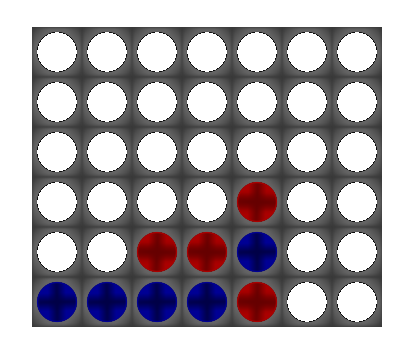
\includegraphics[width=0.4\textwidth]{ejemplo_1.png}
	\caption{(a) Ejemplo de victoria del azul en un 4 en línea tradicional. (b) Ejemplo de empate con $c=3$ y un tablero de $4\times 3$}
\end{wrapfigure}

En los ejemplos de la Figura 1 se pueden observar distintas configuraciones posibles del juego. La Figura 1 (a) muestra un tradicional 4 en línea donde el jugador azul ha conseguido la victoria porque abajo a la izquierda ha conseguido formar una línea horizontal de 4 fichas propias. La Figura 1 (b) es un ejemplo de 3 en línea (no confundir con el nombre español del tatetí) en un tablero de 4 filas y 3 columnas. En este caso se ha dado un empate pues ninguno de los dos jugadores ha podido formar una línea de 3 y ya se ha llenado el tablero.


\section{Jugador Óptimo}

\subsection{El algoritmo}

El algoritmo del jugador del punto 1.a brinda un jugador óptimo. Nos asegura que este jugador hará la estrategia ganadora si hubiera. En caso de que esta no exista, realizará una de empate. Y si tampoco existiera esa, jugará indistintamente sabiendo que perderá. Este análisis se realiza jugada a jugada. Para ejemplificar esto, podría suceder que el oponente tenga la estrategia ganadora y en ese caso nuestro jugador hará cualquier movida indistintamente (pues sabe que perderá), pero si en la próxima jugada el oponente no realiza la correspondiente a su estrategia ganadora y da un nuevo estado del tablero en el que esta vez nuestro jugador tiene estrategia ganadora, nuestro jugador jugará y ganará ya que ahora sí tiene estrategia ganadora.

Para lograr esto, utilizamos una técnica algorítmica similar al Backtracking en el sentido de que exploramos todas las soluciones posibles y nos quedamos con la óptima. Pero esta vez tenemos dos jugadores interviniendo en la situación donde lo que uno busca es todo lo contrario a lo que busca el otro. Podemos decir que un tablero finalizado tiene 3 puntajes posibles, 1 si ganamos nosotros, 0 si es empate, -1 si ganó el otro (podríamos sino generalizarlo para todo tablero y que haya un cuarto valor que sea inválido si aún no hemos calculado el valor de dicho tablero). Así, lo que sabemos es que turno a turno, uno quiere maximizar el puntaje y el otro minimizarlo. Es por esto que dicha técnica algorítmica se llama Minimax. 

De esta manera, igual que en Backtracking tenemos un árbol de ejecución donde cada nodo es un estado del tablero y la raíz es el tablero vacío. Cada nodo (que no sea hoja) tendrá $N$ hijos donde cada uno representará que la próxima jugada fue en alguna de las $N$ columnas. De esta forma, recorremos todos los tableros posibles. Según quién comience, en el primer nivel trataremos de maximizar o minimizar, en el siguiente lo contrario y así sucesivamente. Todos los niveles impares minimizarán si empieza el contrincante y maximizarán si empieza nuestro jugador. El que maximiza le asignará a su nodo un puntaje que será el máximo de los puntajes de todos sus hijos. Análogamente el que minimiza le asignará a su nodo un puntaje que será el mínimo de los puntajes de todos sus hijos.

Así, ejecutando dicho algoritmo la raíz tendrá la información de quién tiene la estrategia ganadora, o que ambos pueden asegurar el empate según quién empiece y haya un 1, 0 o -1. Esta es la idea general del algoritmo, lo veremos más claro en pseudocódigo.

\subsubsection{El Pseudocódigo}
Comenzaremos con el \texttt{main} que es donde se hace el intercambio con el juego en sí. Para ello, primero se le ingresan los parámetros del tablero y las condiciones de juego y luego se desarrolla la partida. Esta termina cuando se lee el mensaje ''ganaste'' ''perdiste'' o ''empataste''. En cada iteración del ciclo (es decir, cada turno) se llama a la función \texttt{minimax} (que se detallará luego y es el algoritmo en sí que resuelve el problema).

Antes del ciclo hay un \texttt{If} que es la ejecución del primer turno si empezamos nosotros a jugar ya que el ciclo comienza con la jugada del otro o la finalización del juego. Esto está determinado por un mensaje que se lee al iniciar el ciclo; si es un número, indica en qué columna jugó el adversario, si es el $string$ ''ganaste'', ''perdiste'' o ''empataste'' termina la ejecución.


\begin{algorithm}
	\texttt{leer} parámetros: \textit{color, oponent\_color, columns, rows, c, p}
	
    inicializar $tablero$

	\texttt{leer} quién empieza

	\If{empiezo yo}
		{
		$movida$ = \texttt{minimax}($rows$, $columns$, $c$, $p$, $tablero$, \textbf{true}, -1).first

		\texttt{AgregarAtras}($tablero[movida]$, 1)

		resto 1 a $p$

		\texttt{jugar}($movida$)		
		}

    \While{$true$}
    	{
    	\texttt{leer} $mensaje$

        \If{el $mensaje$ es de finalización}
        	{
        	\textbf{break}
            }

        \texttt{AgregarAtras}($tablero$[movida del otro jugador], 2)        	

		resto 1 a $p$

        $movida$ = \texttt{minimax}($rows$, $columns$, $c$, $p$, $tablero$, \textbf{true}, -1).first

        \texttt{AgregarAtras}($tablero[movida]$, 1)

        resto 1 a $p$

    	\texttt{jugar}($movida$)
    	}
    \caption{Main}   
\end{algorithm}

El algoritmo del \texttt{minimax} devuelve una tupla de enteros donde el primero es la columna donde se consigue el mejor valor posible, es decir, la jugada  que da resultado óptimo (si existe) desde el tablero de entrada, y el segundo es el mejor valor que se puede conseguir al hacer esa jugada. Se usaron los valores 1, 0 y -1 para asignar los valores respectivos a ganar, empatar o perder. Además, se usó $\infty$ cuando alguno de estos valores estaba indefinido.

\newpage

\begin{algorithm}
	\SetKwInOut{Input}{Input}


    \Input{\textbf{int} rows, \textbf{int} columns, \textbf{int} c, \textbf{int} p, \textit{matriz}(\textbf{int} \textbf{int}) tablero,  \textbf{bool} maximizo, \textbf{int} ultimajugada}
    
		\If{\texttt{gane}}
			{
			\textbf{return} ($\infty$,1)
			}

		\If{\texttt{perdi}}
			{
			\textbf{return} ($\infty$,-1)
			}

		\If{empate porque no hay más fichas}
			{
			\textbf{return} ($\infty$,0)
			}

		\If{empate porque se llen\'o el tablero}
			{
		    \textbf{return} ($\infty$,0)
		    }
		
		mejorColumna = 0

		mejorValorPosible = jugar en cero

		\For{cada jugada posible}
			{
				\eIf{Maximizo}
					{
					\If {valor de esta jugada $>$ mejorValorPosible}
		  	  			{
						mejorColumna=esta jugada

						mejorValorPosible=valor de esta jugada
						}
					}
					{
		   	 		\If {valor de esta jugada $<$ mejorValorPosible}
		  	  			{
						mejorColumna=esta jugada

						mejorValorPosible=valor de esta jugada
						}
					}
			}
		\textbf{return} (columna del máximo, máximo)
		

\caption{Minimax}
\end{algorithm}

Las funciones \texttt{gane} y \texttt{perdi} devuelven \textbf{true} si con la jugada se gana la partida o se pierde, respectivamente. Ambas consisten en llamar a la funcion \texttt{ganoJugador} pasándole como jugador al 1 o al 2 respectivamente. Esta función va verificando las distintas condiciones de victoria para el jugador que se le pasó por parámetro (es decir, si con la última jugada se forma $c$ en línea vertical, horizontal o diagonal) hasta que encuentre alguna devoliendo \textbf{true}. Si no encuentra, devuelve \textbf{false}. Cabe aclarar que llamar al proximo en el arbol de minimax no es mas que llamar nuevamente a minimax (tantas veces como columnas libres haya), donde el tablero que le pasamos es el mismo solo que habiendo jugado en la columna posible en particular que estamos mirando y se cambia el valor de maximizo (si estaba maximizando, el próximo turno será el del jugador que minimza y viceversa), también se decrementa en uno la cantidad total de fichas.



\subsection{Poda $\alpha$ - $\beta$}

La poda $\alpha$ - $\beta$ consiste en disminuir la cantidad de accesos a nodos del árbol de minimax a partir de información obtenida por accesos previos a otros nodos. La idea general es que, si ya si se está evaluando un nodo en el que juega el jugador 1 (es lo mismo con el jugador 2), y por un camino tiene estrategia ganadora, no hace falta recorrer los otros pues, en el mejor de los casos, igualamos el resultado anterior, seguro este jugador no va a encontrar nada que prefiera por sobre este camino.Esta poda también sirve para situaciones en las que un jugador puede garantizar un empate y por lo tanto sabemos que no hay que terminar de explorar ningún nodo en el que su oponente pueda ganar, ya que nunca veremos la situación que ese nodo representa en el partido real, el primer jugador siempre elegirá empatar por encima de darle la oportunidad de ganar a su oponente.

El algoritmo se denomina $\alpha$ - $\beta$ por el nombre de las variables donde se guardan el valor máximo y el mínimo de lo que se puede conseguir hasta el momento. Más precisamente, $\alpha$ es el valor más alto que puede conseguir el jugador 1. Análogamente, $\beta$ es el mínimo valor que puede asegurarse el jugador 2. Es importante aclarar que estos valores no son constantes en todos los nodos del arbol, cada nodo recibe los valores  $\alpha$ - $\beta$ de su padre, pero si juega el jugador 1 solo se actualiza el valor  $\alpha$, que será igual al máximo  $\alpha$ de sus hijos, en cambio  $\beta$ solo se actualiza en los nodos en los que juega el jugador 2 y se calcula como el mínimo $\beta$ de sus hijos. El caso base de esta recursión es el partido terminado, en el que tanto $\alpha$ como $\beta$ toman el valor del tablero final.

Como ejemplo se puede imaginar la siguiente situación: se está analizando un turno del jugador 2, y recibe un $\alpha$ = 0, lo que significa que el jugador 1 en el turno anterior puede conseguir un empate asegurado. Se analizan algunas opciones posibles para el jugador 2, y en una consigue una victoria asegurada, esto significa una derrota para el jugador 1, luego el valor de $\beta$ en este nodo se igualará a -1, ya que es el valor mínimo que puede conseguir el jugador 2 (mínimo desde el punto de vista del jugador 1). En este momento $\beta  \leq \alpha$ lo que significa que el jugador 1 en un turno anterior tiene otra forma de jugar que le devuelve un valor mayor (empate) en lugar de venir a este nodo en el que el jugador 2 se asegurará de conseguir un valor menor (derrota para el jugador 1). El primer jugador entonces nunca llegará a este nodo, y por lo tanto no es necesario explorar las otras posibilidades que tenía el jugador 2 en el mismo, ya que nunca se darán en el partido real.

De este modo, cuando se analice un nodo para determinar el camino máximo, se siguen los mismos pasos detallados en la sección 2.1 pero si en algun momento $\alpha \geq \beta$ sabemos que nunca se llegará verdaderamente a este nodo, porque en alguna jugada anterior algún jugador tiene una opción mejor o igual que ya estudió en su totalidad que venir a esta posición, por lo tanto se ahorra trabajo computacional evitando el análisis de todas las ramas que surgen de este nodo que no va a ser visitado.

En nuestro problema, el número del nodo es 1, 0 o -1 para ganar, empatar o perder (desde el punto de vista del jugador 1), por lo que la poda se puede simplificar diciendo que, si ya se conoce un camino que asegura la victoria a partir de cierto tablero, no hace falta mirar el resto de las opciones que se desprenden de ese tablero, y si ya se conoce un camino que asegura el empate, y en un nodo el oponente tiene estrategia ganadora, no hace falta terminar de estudiar ese nodo ya que siempre se evitará.



\subsubsection{Pseudocódigo}
El código de este algoritmo es en su mayoría igual al detallado en la sección previa, con la única diferencia de ir modificando alfa y beta. Por la similitud que presenta se copiará solamente el chequeo de todas las jugadas posibles dentro del minimax, sabiendo que la función main y los cuatro chequeos para tableros terminales en minimax se mantienen iguales

\newpage

\begin{algorithm}
	\SetKwInOut{Input}{Input}


    \Input{\textbf{int} rows, \textbf{int} columns, \textbf{int} c, \textbf{int} p, \textit{matriz}(\textbf{int} \textbf{int}) tablero,  \textbf{bool} maximizo, \textbf{int} ultimajugada, \textbf{int} $\alpha$, \textbf{int} $\beta$}

		mejorColumna = 0

		mejorValorPosible = jugar en cero

		\For{cada jugada posible}
			{
				\If{ $\alpha >= \beta$}				
					{
					Break
					}

				\eIf{Maximizo}
					{
					\If {valor de esta jugada $>$ mejorValorPosible}
		  	  			{
						$\alpha$ = valor de esta jugada

						mejorColumna=esta jugada

						mejorValorPosible=valor de esta jugada
						}
					}
					{
		   	 		\If {valor de esta jugada $<$ mejorValorPosible}
		  	  			{
						$\beta$ = valor de esta jugada

						mejorColumna=esta jugada

						mejorValorPosible=valor de esta jugada
						}
					}
			}
		\textbf{return} (columna del máximo, máximo)
		

\caption{Minimax}
\end{algorithm}


\subsection{Complejidad}

Veremos que la complejidad es $\mathcal{O}(a^b)$ donde $a=|Columnas Donde Es Posible Jugar|$ y $b =$ mín $\{|FichasRestantes|$, $|Casillas Libres En El Tablero|\}$ que es en particular acotable por $\mathcal{O}(N\textsuperscript{NM})$ ya que a lo sumo se puede jugar en $N$ columnas (no hay más en el tablero) y a lo sumo hay $N*M$ casillas libres (o sea, el tablero esta vacío). Cabe aclarar que \textit{fichas restantes} son la fichas restantes totales (las mías + las suyas). Esto es porque el algoritmo de \texttt{minimax} es como un árbol de \texttt{Backtracking} en el sentido de que checkea todas las posibles sucesiones de jugadas que se pueden dar, considerando tanto lo que yo juego como lo que él juega.

Si bien en total hay menos de $3\textsuperscript{NM})$ tableros posibles (cada casilla puede estar vacía, o tener una ficha de alguno de los dos jugadores, y acota por arriba pues hay casos que no son posibles, como que haya una ficha encima de una vacía) esto no cuenta la cantidad de posibles partidas que se pueden dar, ya que un mismo tablero podría ser alcanzado de varias formas. Pero a cada paso, cada jugador tiene $N$ opciones de jugada y a lo sumo se juega $N*M$ veces (se llena el tablero) y por ende tenemos $N\textsuperscript{NM}$ estados posibles del tablero. Lo que hace el algoritmo es para cada uno de estos tableros, evaluar si hay o no un ganador y en base a eso establecer un puntaje al tablero que es el que transmite \texttt{minimax}. Este checkeo tiene un costo de $\mathcal{O}(c)$ ya que la función, por cómo fue implementada, recibe cuál fue la última jugada y sabe cómo se empata o si con la última jugada se logra que algún jugador gane. Además, checkear las primeras dos condiciones es $\mathcal{O}(1)$ sabiendo la cantidad de fichas que quedan y de filas y columnas (que es un dato que se pasa por parámetro). Pero si gano con esa ficha solo hay que verificar las $c$ fichas para todos los sentidos y direcciones (8 en total, 4 direcciones con sus dos sentidos cada una), lo que es $8 \mathcal{O}(c)= \mathcal{O}(c)$. 

Luego, dado un tablero, conociendo el valor de minimax de sus hijos, queda tomar máximo o mínimo según corresponda. Pero como tiene $N$ hijos a lo sumo (si no es hoja) ya que son las $N$ posibles jugadas inmediatas, esto es $\mathcal{O}(N)$. Esta operación la hacemos para todo nodo (como también checkear si hay un ganador). Por lo tanto, la complejidad total resulta $|Nodos|\mathcal{O}(N)\mathcal{O}(c)$, y ya se ha visto que $|Nodos|=a^b$ por lo que se obtiene una complejidad $\mathcal{O}(N c a^b)$ lo que es acotable, como se ha visto por $\mathcal{O}(N c N\textsuperscript{NM})=\mathcal{O}(c N\textsuperscript{(N+1)M})$. Pero si recordamos que $c<$ mín$\{N,M\}$ podemos deducir que la complejidad es menor que $\mathcal{O}(N\textsuperscript{((N+1)M)+1})$.

En cuanto a la complejidad del algoritmo con poda, no hay modificaciones ya que la misma cota es válida puesto que la única diferencia que tiene la poda es que guarda registro de dos valores ($\alpha$ y $\beta$) y los compara a cada paso, lo que es $\mathcal{O}(1)$ y por ende no afecta la complejidad. Si bien la poda corta varias ramas del árbol de minimax, no podemos asegurar una cota de cuántas ramas cortará y por ende, la complejidad teórica seguirá siendo la misma. Sin embargo uno espera que la poda se ejecute y varias ramas no se checkeen, reduciendo así el tiempo de ejecución en comparación con el algoritmo sin poda.



\subsection{Experimentación}

\subsubsection{Contexto} 


La experimentación se realizó toda en la misma computadora, cuyo procesador era Intel Atom\texttrademark CPU N2600 @ 1.60GHz, de 36 bits physical, 48 bits virtual, con una memoria RAM de 2048 MB.  Para experimentar, se calculó el tiempo que tardaba el algoritmo sin considerar el tiempo de lectura y escritura ni el tiempo que llevaba armar la matriz (ya que se leía un dato, se escribía la matriz y luego se leía el siguiente). 

El tiempo se medía no como tiempo global sino como tiempo de proceso, calculando la cantidad de ticks del reloj (con el tipo \texttt{clock\_t} de C++) y luego se dividía el delta de ticks sobre\texttt{ CLOCKS\_PER\_SEC}. En todos los experimentos el tiempo se mide en segundos. El contexto de experimentación será el mismo a lo largo de todo el trabajo.

\subsubsection{Sin poda}
En principio, para verificar experimentalmente que el jugador era óptimo se jugó en tableros pequeños (en particular, de $2\times2, 3\times3, 2\times3, 3\times2, 2\times4, 4\times2, 3\times4, 4\times3$) con un $c=2, 3, 4$ siempre que cumpla la condición del juego ($c\leq min\{N,M\}$) contra el jugador random. En todos los casos la cantidad de iteraciones fue de $2*3\textsuperscript{NM}$ por lo que todo tablero posible tenía una probabilidad considerable de ser jugado (notar que la cantidad de juegos posibles es menor que $N\textsuperscript{NM}$ -de hecho es menor que $3\textsuperscript{NM}$ ya que cada casilla tiene o bien nada o ficha de un jugador o del otro-). Tomamos esta cantidad de repeticiones ya que a cada paso lo que se elige es una de $N$ -o menos si hay columnas llenas- opciones donde jugar y esto se repite hasta que termine el juego -a lo sumo se lena la grilla $N*M$ veces-. Así, tenemos tantas iteraciones como secuencias posibles de jugadas, o sea partidas en general. Como el jugador es random equiprobable, la distribución respecto de qué jugada de las posibles realizar es uniforme y lo multiplicamos por 2 para que sea más probable que salga cualquier partida posible (estamos jugando toda partida posible con una probabilidad considerable). Más aún, es una probabilidad bastante alta ya que se puede notar que solo queremos contar todas las opciones de secuencias de jugadas que puede dar el segundo jugador (en este caso el aleatorio), lo que nos provee una cota menor de la cantidad total de jugadas distintas que se le pueden hacer al jugador optimo, acotándolo por $N^{ \frac{NM}{2} }$.

Estos experimentos se repitieron en dos casos cada uno, cuando comenzaba el \texttt{minimax} y cuando comenzaba el random. Además para fijado el jugador que empieza, se repitió con valores de fichas que fueron $p=\frac{NM}{2}, \frac{NM}{3}, \frac{NM}{4}$ donde el primer valor de $p$ aseguraba que se pueda jugar sin límite de fichas (siempre se podría llegar a llenar el tablero) y los otros dos sí imponían un limite de fichas. Luego de cada experimento, nos fijamos en el archivo \texttt{.log} devuelto por dichas iteraciones y en todos se observó el mismo comportamiento:
\begin{itemize}
\item O bien siempre ganaba (lo que nos indica que había estrategia ganadora para el que empieza). Al invertir la situación (cambiando el jugador que empieza), se daba el ítem 3.
\item O bien siempre ganaba o empataba (lo que nos indicaría que la mejor estrategia para ambos resulta en un empate, pero como el jugador random no siempre juega lo mejor, le daba la posibilidad a nuestro jugador de ganar). Al invertir la situación (cambiando el jugador que empieza) se obtenía la misma situación, este mismo item, o sea, siempre ganaba o empataba (lo que indicatía que la mejor estrategia para ambos resulta en un empate).
\item O bien siempre ganaba o empataba o perdía (lo que nos indicaría que el que no empieza tiene estrategia ganadora, pero como el jugador random no siempre juega lo mejor, le daba la posibilidad a veces a nuestro jugador de ganar). Al invertir la situación (cambiando el jugador que empieza), se daba el ítem 1.
\end{itemize}

Como se explicó, estas situaciones, en todos estos tableros, reforzaron fuertemente la idea de que se trataba de un jugador óptimo. Cabe aclarar que se realizó solo con tableros pequeños debido a que, para tableros muy grandes el jugador demoraba demasiado tiempo en decidir que jugar (como se vio en la complejidad teórica exponencial, por lo que crecía brutalmente al crecer el tamaño del tablero y la cantidad de columnas) y por ende resultaba inviable realizar una alta cantidad de iteraciones para recorrer una gran cantidad de tableros posibles lo que nos permita reforzar la idea de optimalidad del jugador. 

Pero en tableros pequeños hemos podido comprobar que en todos los tableros que se dieron, cumplieron que el jugador era óptimo ya que si tenía la posibilidad de ganar lo hacía, en caso de que esta no existiera, si tenía la posibilidad de empatar lo hacía y recién en caso de no existir, jugaba cualquier cosa sabiendo que perdería. Pero como hemos visto, esto se comprobaba paso a paso, por lo que el jugador podía jugar creyendo que perdería y, como el otro no jugó optimamente luego, pasar a poder ganar o empatar (y efectivamente hacerlo pues es óptimo); o sea, asume optimalidad del rival.

Esta experimentación nos permitió reforzar nuestra idea (al menos para estos tableros pequeños y con una probabilidad muy alta) de que el jugador era efectivamente óptimo.

Para tratar de reforzar experimentalmente la complejidad teórica deducida previamente, se realizó una experimentación en la que se registró para varios tableros de tamaño pequeño (de $2\times2, 3\times3, 4\times4, 2\times3, 3\times2, 2\times4, 4\times2, 5\times2, 2\times5, 2\times6, 2\times7, 2\times8, 6\times2, 7\times2, 8\times2, 3\times4, 4\times3, 3\times5, 5\times3$) ya que para tamaños mayores los tiempos de ejecución fueron inabordables (lo que reforzó en parte la complejidad teórica esperada). Para cada uno de esos tableros, se jugó con fichas de sobra (más que la cantidad que entraba en el tablero, 88 particularmente) y el $c$ se movió entre $2, 3$ y $4$ siempre y cuando se cumplieran las condiciones del juego. Además, siempre se jugó contra el jugador random provisto por la cátedra (que con distribución uniforme decidía aleatoriamente en cuál de las $N$ posibles columnas jugar). Para asegurar distintas configuraciones, se repitió cada partido $10$ veces. 


Para todos estos juegos se registró a cada jugada del algoritmo el tiempo de ejecución que este tomó en decidir qué jugada realizar y se registró una variable que reflejaba un refinamiento de la complejidad esperada. Esta variable se definió como $Nca^b$ donde $a=|Columnas Donde Es Posible Jugar|$ y $b =$ mín$\{|FichasRestantes|$, $|Casillas Libres En El Tablero|\}$ que es en particular acotable por $cN\textsuperscript{(N+1)M}$. Luego, se graficó el $\frac{tiempo}{Nca^b}$ en función de $Nca^b$. Se esperaría obtener un gráfico acotable por una constante que reforzaría la idea de que el aloritmo cumple la cota propuesta. Se graficó, pues, esto en la Figura 2, (junto con su análogo con el algoritmo con poda) y efectivamente se cumplió con lo esperado ya que se ve que el gráfico es prácticamente constante salvo en los primeros valores, lo que tiene sentido y refuerza aún más la hipótesis, porque para esos valores toman mucha más importancia los términos constantes que no dependen de la variable propuesta como complejidad. Al aumentar la variable propuesta, la importancia del término constante se reduce y pasa a ser constante. Más aún, esa constante es $0$, lo que nos indica que es incluso menor a la complejidad propuesta (o sea que cumple lo pedido, ya que en particular es menor, que es a lo que apunta la notación $\mathcal{O}$) ya que este método de dividir por la complejidad esperada es muy sensible, ya que da una constante si dividimos por algo que cumpla ser $\mathcal{\theta}$, y sino ante una pequeña alteración en la complejidad se refleja claramente en el gráfico (o bien pasa a ser creciente o decreciente). Tiene sentido que sea menor ya que muchas veces el partido termina antes de que completemos efectivamente el tablero (que es la cota que propusimos) y además no siempre tenemos tantas opciones como columnas posibles de jugar ahora (cota que propusimos), sino que con el desarrollo del juego las opciones de columnas posibles van disminuyendo. Igualmente, esto nos permite reforzar claramente nuestra hipótesis de que cumple la complejidad teórica propuesta.

\subsubsection{Con poda}
En el caso con poda se realizó la misma experimentación para comprobar la optimalidad. Como el algoritmo tardaba un poco menos (por la poda realizada), se realizó (además de con los ya mencionados) con tableros de tamaño $4\times4, 3\times5, 5\times3, 4\times5, 5\times4, 3\times6, 3\times7$ , con los mismos valores de $c$ que antes (siempre y cuando cumpliera las condiciones del juego). También se varió la cantidad de fichas de la misma forma.

Nuevamente, los resultados y conclusiones sobre estos fueron los mismos, lo que nos permitió reforzar nuestra idea (al menos para estos tableros pequeños y con una probabilidad muy alta) de que el jugador era efectivamente óptimo.



\begin{wrapfigure}{R}{0.4\textwidth}
	%\centering
	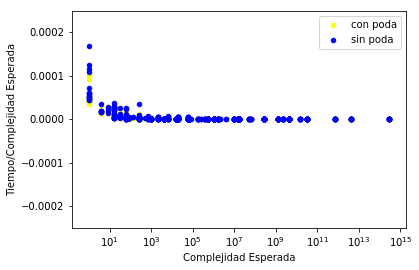
\includegraphics[width=0.4\textwidth]{complejidad1.png}
	\caption{ Gráfico de segundos de ejecución (de cada jugada) dividido $N*c*a^b$ en función de $N*c*a^b$ para los partidos jugados por el algoritmo con y sin poda en tableros pequeños contra el jugador random.}
\end{wrapfigure}


Para verificar que la poda efectivamente se ejecutaba y permitía podar varios niveles del árbol de ejecución del minimax, decidimos analizar el tiempo de ejecución ya que si no se analizaran estas partes podadas, el tiempo de ejecución sería menor. Por eso se ejecutó para exactamente las mismas partidas con las que se experimentó sin poda, la misma cantidad de veces cada una, contra el mismo jugador (que era el jugador random) que es importante aclarar que como no era determinístico medimos en la misma partida (o sea, ambos algoritmos -con y sin poda- recibían el mismo tablero a cada jugada) el tiempo de ejecución de ambos (y finalmente jugaba el ''con poda'' la jugada -lo que nos resultaba poco relevante ya que queríamos medir tiempos de ejecución para distintos tableros y verificar nuestra complejidad que no dependía de cómo jugaban y tampoco era el objetivo analizar como jugaban-). Luego se compararon los dos tiempos medidos para las 688 jugadas en todos los partidos. Así, solamente fueron 9 jugadas en las que el algoritmo con poda tardó más que el sin poda y estas diferencias fueron realmente despreciables (tanto en cantidad de jugadas diferentes, como en diferencia de tiempo). Listamos a continuación los valores en los que difirieron (5.8e-05 contra 5.6e-05, 0.000383 contra 0.000352, 0.000212 contra 0.000202, 0.000535 contra 0.000251, 0.000282 contra 0.00027, 0.00028 contra 0.000264, 0.000469 contra 0.000459, 0.000417 contra 0.000355, 0.000341 contra 0.000323 -del algoritmo con poda contra el sin poda respectivamente-).

Esta experimentación nos permitió no solo reforzar nuestra hipótesis (justificada teoricamente en el algoritmo) de que el tiempo de ejecución era efectivamente menor, por lo que se ejecutaba la poda, sino también comprobar que se seguía manteniendo la complejidad teórica propuesta para el algoritmo con poda (ya que era la misma que la del algoritmo sin poda y hemos visto que el tiempo de ejecución era menor). Más aún esto se puede ver en la Figura 2 donde se ve que el algoritmo con poda nunca supera al algoritmo sin poda en tiempo de ejecución.



















\section{Jugador parametrizable}


\subsection{El algoritmo}
El algoritmo consiste básicamente en establecer un sistema de puntos para cada tablero, donde se miden solamente ciertas características que decidimos nosotros. A cada una de esas características se le asignará una importancia. El jugador es goloso en el próximo paso, o sea, evalúa todas las opciones que tiene para jugar (todas las columnas donde se puede jugar) y se queda con la que tenga un tablero que le dé el mayor puntaje. La libertad que tiene el jugador es la importancia de cada característica, que es lo que luego se buscará optimizar. Las características que decidimos considerar para ambos jugadores fueron:

\begin{itemize}
\item cantidad de fichas en la columna central, en algun borde, en alguna esquina;
\item la suma de la cantidad de casillas libres al rededor de una ocupada por un jugador (libertades);
\item cantidad de fichas consecutivas de tamaño $1,2,..,c-1$;
\item cantidad de fichas consecutivas de tamaño $1,2,..,c-1$ que se pueden extender (es decir, que tengan al lado casilleros vacíos); 
\item cantidad de fichas consecutivas de tamaño $1,2,..,c-1$ que se pueden extender en el próximo turno (extensiblesprox);
\item cantidad de fichas consecutivas de tamaño $1,2,..,c-1$ que se pueden extender en ambos sentidos (biextensibles).
\end{itemize}
\subsubsection{El Pseudocódigo}
En el \texttt{main} a la variable $movida$ se le asigna el resultado de la función \texttt{parametrizable} que es el algoritmo goloso propuesto para esta parte del problema. Esta toma los mismos parámetros que \texttt{minimax} con el agregado del conjunto de \textbf{parametros} $params$ y devuelve el número de columna donde se debe jugar.

La idea es que se asigne un puntaje a cada tablero y de las opciones posibles (tantas como columnas libres) se tome la de mayor puntaje (esta sería la parte golosa).

En la función se llama a la función \texttt{puntaje} que se verá luego.

La variable $tablero$ se pasa por referencia.
\begin{algorithm}
	\SetKwInOut{Input}{Input}


    \Input{\textbf{int} rows, \textbf{int} columns, \textbf{int} c, \textbf{int} p, matriz(\textbf{int}, \textbf{int}) tablero, \textbf{int} ultimajugada, cjto(\textbf{parametro}) params}
    
    	$posibles = [0,..,columnas-1] -$ las columnas llenas del $tablero$

    	\For{$i \leftarrow [0,..,\lvert posibles \rvert$)}
    		{

    		\If{jugando $posibles[i]$ se evita perder en la siguiente jugada}
    			{
    			\textbf{return} $posibles[i]$
    			}
    		}

    	\textbf{float} $maximoPuntaje =$ \texttt{puntaje}($rows$, $columns$, $c$, $p$, $tablero$, $posibles[0]$, $params$)

    	\textbf{int} $maxpos = posibles[0]$
    	
    	\For{$q \leftarrow [1,..,\lvert posibles \rvert$)}
    		{

			\texttt{AgregarAtrás}($tablero[posibles[q]]$, 1)

			\If{\texttt{puntaje}($rows$, $columns$, $c$, $p$, $tablero$, $posibles[q]$, $params$)$> maximopuntaje$}
				{
				actualizar $maximopuntaje$ y $maxpos$
				}

			Sacarle el último a $tablero[posibles[q]]$		
			}

		\textbf{return} $maxpos$
    
    
    \caption{parametrizable}

\end{algorithm}


La función \texttt{puntaje} devuelve un entero asociado a cierta jugada que se pasa como input (es decir, no solo se pasa la columna donde se se juega, sino también, el tablero con las fichas). La función en sí consiste simplemente en sumar ciertos parámetros asociados a características del estado actual del juego donde el peso de cada uno de esos parámetros esta dado por valores que toma como entrada (que es lo que luego buscaremos optimizar). Por ejemplo, como no es lo mismo tener una ficha en el centro que en un borde, la variable asociada a la cantidad de fichas del centro tendrá distinto peso que la del borde. De este modo, se cuentan ĺos distintos parámetros asociados al tablero actual tanto para el jugador 1 como para el 2. Finalmente, entonces, se devuelven las cantidades del jugador 1 y se le restan las del jugador 2 (pues son las características del estado asociado al oponente).

Previamente se verifica si con la jugada se gana o no. Si es así, el puntaje es $\infty$ así claramente es el máximo y la función anterior lo elige como jugada.

La variable $tablero$, como en \texttt{parametrizable} también se pasa por referencia pero como \texttt{const}.
\begin{algorithm}
	\SetKwInOut{Input}{Input}


    \Input{\textbf{int} rows, \textbf{int} columns, \textbf{int} c, \textbf{int} p, matriz(\textbf{int}, \textbf{int}) tablero, \textbf{int} ultimajugada, conj(\textbf{parametro}) params}
 

		\If{\texttt{gane}}
			{
			\textbf{return} $\infty$
			}    	

    	contar los que estan en el borde de cada jugador
    	
    	contar libertades de cada jugador

    	contar la cantidad de fichas que estan en una esquina de cada jugador

    	contar la cantidad de fichas en el centro de cada jugador

		contar la cantidad de casillas libres alrededor de cada ficha de cada jugador

		contar la cantidad de fichas consecutivas de cada jugador

		contar cantidad de inmediatemente extensibles en la próxima jugada de cada jugador

		contar cantidad de  extensibles en cualquier momento de cada jugador

		contar cantidad de  bi-extensibles (extensibles en ambos sentidos) en cualquier momento de cada jugador

		\textbf{return} $\sum$ cantidad$_{jugador1}*$(puntaje del parámetro)-cantidad$_{jugador2}*$(puntaje del parámetro)
		
		
    \caption{puntaje}

\end{algorithm}

Cabe aclarar que contar la cantidad de fichas en determinadas posiciones es simplemente recorrer el tablero en búsqueda de esas posiciones. De forma similar, contar las consecutivas es mirar todas las filas, columnas y diagonales que hay en el tablero y recorrerlas, contando las consecutivas de un jugador (que es recorrer todo el tablero 4 veces, una horizontalmente, otra vertical, una en diagonal desde arriba a la izquierda, hacia abajo a la derecha y la última en diagonal desde arriba a la derecha, hacia abajo a la izquierda). Teniendo esto en cuenta es simple chequear si cada una de estas tiras es extensible o bi-extensible, viendo simplemente si sus casillas por donde podrían seguir están vacías o no (si existen, cosa que podría no suceder en caso de estar en el borde del tablero) y para ver si son extensibles en el proximo turno es cuestión de analizar si estas casillas tienen debajo alguna ficha o son la primera de su columna (o sea, si se puede jugar ahí en el próximo turno).

\subsection{Complejidad}

Veamos que el jugador que presentamos decide que jugada realizar en tiempo $\mathcal{O}(N^2 M)$ que es menor que $\mathcal{O}(N^2 M^2)$ y por ende, cumple la complejidad pedida. 





En primer término, veamos que calcular el puntaje de un tablero es $\mathcal{O}(NM)$ puesto que lo único que hacemos es recorrer todas las filas, columnas y diagonales (que en total son 4, aunque no importa verdaderamente cuánto sino que es una cantidad constante) y en cada una de ellas contamos cuántas fichas son nuestras y cuántas de él. Pero esto lo repetimos una vez por cada parámetro que tenemos. Como tenemos finitos (y constantes) parámetros, pasamos a recorrer una cantidad constante de veces el tablero. Esto es porque recorrer el tablero es $\mathcal{O}(NM)$ ya que para cada sentido de recorrida, pasamos solo una vez por cada casilla, o sea recorremos $N*M$ casillas; repitiendo esto una cantidad constante de veces (la cantidad de parámetros) y para una cantidad constante de sentidos (cuatro) nos da que recorrimos una cantidad constante de veces $N*M $ casillas, por lo que la complejidad de calcular el puntaje es efectivamente $\mathcal{O}(NM)+\mathcal{O}(c)=\mathcal{O}(NM)$ puesto que $c<$ mín$\{N,M\}$.Además, chequeamos si ganamos o perdimos, que como ya hemos visto en la complejidad del jugador óptimo es $\mathcal{O}(c)<\mathcal{O}(N)<\mathcal{O}(NM)$, lo que no afecta la complejidad.

Cabe aclarar aquí que consideramos como un parámetro a los vectores de parámetros (como es el caso de consecutivos) ya que para ellos recorremos solo cuatro veces el tablero (en todos los sentidos) y lo que cambia es dónde alojamos cada valor del vector según cuántas fichas consecutivas encontremos del mismo color. Cabe aclarar también que la operación para saber qué ficha está en una casilla es $\mathcal{O}(1)$ porque guardamos al tablero en una matriz. Esto es fundamental para poder asegurar la complejidad pedida.

 
Pero nuestro jugador no hace solo eso, sino que analiza cómo quedaría el puntaje del tablero para cada una de sus $N$ posibles jugadas y luego se queda el máximo de ellas (esta es la parte golosa). Repite entonces $N$ veces algo  $\mathcal{O}(N M)$ por lo que da una complejidad de $\mathcal{O}(N^2 M)$ y luego calcula el máximo sobre $N$ elementos que suma $\mathcal{O}(N)$ (es recorrer linealmente un vector) y da una complejidad total de $\mathcal{O}(N^2 M) +\mathcal{O}(N) = \mathcal{O}(N^2 M)$.

\subsection{Experimentación}


\begin{wrapfigure}{L}{0.4\textwidth}
	%\centering
	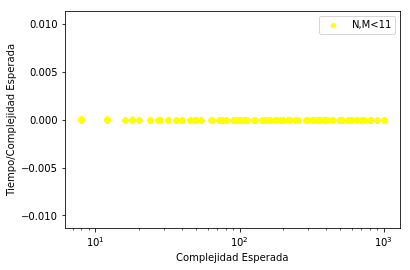
\includegraphics[width=0.4\textwidth]{complejidad2.png}
	\caption{ Gráfico de segundos de ejecución (de cada jugada) dividido $N^2 M$ en función de $N^2  M$ para los partidos jugados por el jugador que utiliza la función parametrizable a cada paso. Varian $c$ y $p$. Columnas y filas menores a 11.}
\end{wrapfigure}

Si bien el grueso del análisis y experimentación sobre este jugador consistirá en buscar buenos parámetros que mejoren al jugador, consideramos relevante reforzar experimentalmente nuestra hipótesis de complejidad teórica esperada. Para esto tomamos mediciones análogas a las del jugador óptimo solo que jugando en más tableros. Se jugó en tableros que comprendían todas las combinaciones factibles con las columnas y filas moviéndose entre $2$ y $10$, $c$ moviendose entre $2$ y mín$\{columnas,filas\}$ y $p$ moviéndose entre $2$ y $filas*columnas/2$. En cada jugada, los parámetros que determinaban la próxima jugada a realizar se sorteaban aleatoriamente. Todo esto fue para ver experimentalmente que la dependencia que proponíamos en la complejidad dependía efectivamente solo de $n$ y $m$. Así, igual que antes, realizamos un gráfico de $\frac{tiempo}{filas*columnas^2}$) en función de $filas*columnas^2$ donde esperábamos obtener un gráfico constante que reforzaría nuestra hipótesis de que la complejidad (como se justificó teóricamente) era de $\mathcal{O}(N^2 M)$. Este gráfico se puede ver en la Figura 3.




Efectivamente, como se puede ver en la Figura 3, pareciera cumplirse la complejidad esperada ya que el gráfico es practicamente constante. Más aún, al variar por todas sus posibilidades $c$, $p$ y el parámetro de la función, esto refuerza la hipótesis (que se justificó en la explicación del algoritmo) de que esta cota de dependencia no se ve afectada por el parámetro en particular, o la cantidad de fichas que queden, o el $c$. Sabiendo esto, tenemos la posibilidad de experimentar para tableros de mayor tamaño (ya que no tenemos que repetirlos para distintos $c$ y $p$). Por esto, se experimentó con un $c$ aleatorio (con distribución uniforme, usando \texttt{rand()} de C++) entre 2 y mín$\{columns,rows\}$, y $p=N\frac{M}{2}$ para que no se interrumpa el partido por falta de fichas y se varió nuevamente las filas y columnas pero con el límite superior igual a 20 en vez de 10. Nuevamente, se realizó el mismo gráfico que antes con los nuevos , que se puede ver en la Figura 4.

\begin{wrapfigure}{R}{0.4\textwidth}
	%\centering
	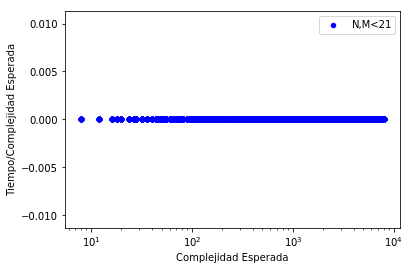
\includegraphics[width=0.4\textwidth]{complejidad2b.png}
	\caption{ Gráfico de segundos de ejecución (de cada jugada) dividido $N^2 M$ en función de $N^2  M$ para los partidos jugados por el jugador que utiliza la función parametrizable a cada paso. Columnas y filas menores a 51.}
\end{wrapfigure}

Podemos ver en el gráfico de la Figura 4, que los resultados siguen siendo los mismos incluso para tableros de tamaño mayor. Nuevamente el gráfico es prácticamente una constante. El análisis y su justificación es totalmente análogo al realizado en la Figura 3 y al ser con tamaños de entrada mayores, refuerza más aún experimentalmente la complejidad que fue propuesta teóricamente.






\section{Grid Search}



\subsection{El algoritmo}

Para mejorar el rendimiento del jugador se implementó, en primer lugar, un \texttt{grid search}. Esta técnica consiste en tomar el conjunto de parámetros que definen una instancia del jugador y buscar la combinación óptima de valores de dichos parámetros. Para ello, se define, en primer lugar, un intervalo para cada parámetro por el cuál se buscará el resultado. En nuestro caso, se eligió usar el mismo para todos, el intervalo $[-1,1]$. Esto es porque al tener finitos parámetros, podríamos dividir a todos por el de numero mayor y poner a todos en dicho intervalo (porque por nuestra eleccion de los parametros, estos siempre multiplican, por lo que dividir a todos por la misma constante mantiene la relacion). Ahora bien, como este espacio es muy grande, para buscar individualmente cuál es mejor, se lo discretiza tomando saltos de a $0.1$. De este modo, para cada parámetro, se recorrieron, en principio, los valores $-1, -0.9,-0.8,...,1$ (fue nuestra forma de discretizar el espacio, podria elegirse otros saltos). 

Una forma más precisa de verlo es con una grilla (de ahí el nombre del algoritmo) de $n$ dimensiones (con $n$ la cantidad de parámetros) donde cada fila o columna $n$-dimensional es un valor fijo de un parámetro. Pensándolo solo con 2 parámetros, las filas corresponderían a los valores $-1, -0.9...$ de un parámetro y las columnas a sendos valores del otro. Cada casilla representaría el resultado obtenido de jugar con el conjunto de parámetros dado por esa fila y columna. De este modo, si se recorre la grilla completa se puede encontrar el valor óptimo y, por consiguiente, la mejor combinación de parámetros.

En principio, para determinar cuándo una combinación es mejor que otra simplemente se enfrentan los dos jugadores y, quien resulta ganador es porque presenta una mejor combinación de parámetros. Esta combinación ganadora se guarda en la variable $mejor$ que se irá actualizando cada vez que un nuevo conjunto de parámetros juegue mejor que él. Cabe aclarar que, como los jugadores son deterministas, con solo dos enfrentamientos alcanzan (invirtiendo quién empieza a jugar), pues, para idénticos parámetros se desarrollarán idénticos juegos. Un jugador se considera mejor que otro si y solo si ganó al menos una vez y nunca perdió.
 
\subsubsection{El Pseudocódigo}

\begin{algorithm}
\SetKwInOut{Input}{Input}


\Input{\textbf{int} rows, \textbf{int} columns, \textbf{int} c, \textbf{int} p, cjto(\textbf{parametro}) params}

cjto(\textbf{parametro}) $mejor$

\For{$i \leftarrow [1..\lvert params\rvert]$}
	{
	\For{$j \leftarrow [-1,-0.9,-0.8,..,1] $}
		{	
		\If{jugador($p_i +j$) $>$ jugador($mejor_i$)}
			{		
			$mejor_i = p_i +j$		
			}
		}
	}

\textbf{return} $mejor$

\caption{Grid Search}
\end{algorithm}

\subsection{Experimentacion}

\subsubsection{Primera exploración}

La primer idea que surge al comenzar la experimentación computacional del método heurístico con\texttt{ grid search} es que a causa de la cantidad de parámteros (28 para el 4 en línea) que tiene en cuenta la función paramétrica detallada en la sección 3, resulta demasiado costoso computacionalmente explorar todo el espacio de posibilidades con un\texttt{ grid search} clásico. Incluso, con una granularidad muy baja, comparando entre tan poco como 20 valores posibles para cada parámetro (cada uno en [-1,1] con saltos de 0,1) se deben analizar $ 20^{28}$ combinaciones de parámetros distintas. Por esto, en lugar de utilizar el algoritmo detallado en la sección 4.1, como era la idea original, se recurrirá a una modificación del mismo para acelerar el tiempo de ejecución.

A causa del tamaño inabarcable del espacio de búsqueda se decidió entonces utilizar un método que reduce de forma drástica el tiempo necesario para obtener resultados del\texttt{ grid search}, con el conocimiento de que no se podrá explorar todo el espacio de esta forma. Empezando con un conjunto de parámetros aleatorios fijo, se buscaba con el método de\texttt{ grid search} la configuración óptima únicamente para los primeros dos parámetros. Una vez que se encontraron los valores óptimos para los primeros dos parámetros en el contexto del conjunto aleatorio inicial, se procede a optimizar el próximo par de parámetros pero manteniendo los mejores valores encontrados para el par ya explorado. Esto se repite hasta optimizar todos los parámetros a tener en cuenta. La desventaja de este método es que a medida que se van modificando los valores de pares, las optimizaciones iniciales van perdiendo relevancia, ya que no tienen por qué ser las óptimas para esta nueva configuración.

Este primer intento no dio buenos resultados. El jugador resultante no realizaba las jugadas esperadas y al enfrentarlo 1000 veces contra un jugador aleatorio ganaba un porcentaje similar al de un jugador con parámetros aleatorios, esto nos muestra que el algoritmo de optimización no cumplió con su objetivo.


\subsubsection{Modificaciones}

En busca de mejores resultados se realizaron los siguientes cambios para mejorar el conjunto de parámetros resultante de ejecutar el \texttt{grid search} con un jugador inicial aleatorio al cual se le van optimizando un par de parámetros a la vez. El primer cambio fue simplemente iterar la versión anterior varias veces, aprovechando que recorrer matrices de solo 2 dimensiones hace al algoritmo más rápido. Como siempre se guarda el mejor jugador hasta el momento y se lo suplanta únicamente si se encontró otro conjunto de parámetros mejor, realizar más iteraciones en el peor caso mantendría la misma solución. El objetivo de este cambio sería darle otra oprtunidad a los parámetros a optimizarse en este nuevo contexto en el cual las otras preferencias del jugador no son las iniciales aleatorias, sino unas calculadas en base a este mismo algoritmo. 

Otra modificación fue poner los parámetros que consideramos más importantes (la cantidad de filas biextensibles grandes, por ejemplo) más adelante en el orden en que se chequean, es decir que se optimicen primero, antes de tocar los otros parámetros aleatorios. De esta forma, se intenta dejarlos buscar su configuración óptima sin estar condicionados por los valores convenientes para otros parámetros menos importantes. 

Puede verse que esta última modificación es importante si se tiene en cuenta lo siguiente: los valores de los parametros en nuestra implementación están acotados en el conjunto [-1,1], por lo tanto si al valor que determina la preferencia del jugador por poner fichas en las esquinas se lo optimiza primero, como todos los otros valores son aleatorios podría ser que el resultado óptimo para esta preferencia de jugar en las esquinas sea muy alto, cercano a 1. Si esto ocurriera, cuando se llegara a intentar optimizar otros valores en principio más importantes, como la importancia de cadenas biextensibles de tamaño $c-1$ no tendría la posibilidad de darle una importancia mayor a la de jugar en las esquinas, ya que no podría pasarse de 1. Esto presenta un problema ya que sabemos que un jugador bueno seguramente debe tener ciertos valores en grados de magnitud mayores que otros. Es importante aclarar que aunque no se acotaran los valores entre [-1, 1] no se evitaría el problema ya que los límites a la hora de implementar el algoritmo fuerzan inevitablemente una cota superior sobre los valores elegidos.

Incluso con las modificaciones a la idea original, la forma de recorrer la grilla de a pares de parametros resultaba muy acotada, y no llegaba a encontrar buenas combinaciones de valores que resultaran en un jugador bueno, al enfrentarlo a un jugador aleatorio su porcentaje de victorias no presentaba mejora en comparación con la idea original. Esto es de esperar ya que si recordamos el tamaño gigante de $ 20^{28}$ posibilidades no hay manera de explorarlo en su completitud en un tiempo razonable, por lo tanto en lugar de recorrerlo a partir de un conjunto de parametros aleatorios es intentaremos guíar la exploración con una solución inicial. A causa de esto se recurrió a la posibilidad de comenzar el\texttt{ grid search} no con un conjunto de parámetros aleatorios, si no con un jugador hecho ''a mano'', con parámetros medianamente buenos. Con esto se buscaba que el\texttt{ grid search} explore opciones cercanas a un conjunto que ya se sabe que no es muy malo. De este modo se intentó evitar la gran cantidad de combinaciones inútiles que el algoritmo estaba recorriendo previamente, y en su lugar mejorar una solución inicial.



\subsubsection{Grid recomendado}


Con la recomendación de parámetros iniciales se esperaban observar resultados mejores del\texttt{ grid search}. El jugador resultante surge de haber vencido a los valores de entrada, por lo cual no sólo debería tener un nivel de juego muy superior a los intentos previos del algoritmo, sino que debería ser mejor que el parámetro que le dimos inicialmente (el hecho por nosotros, '' a mano ''). El problema surge en este punto, a causa de la naturaleza compleja del juego, resulta difícil especificar exactamente \textit{qué} define a un mejor jugador. ¿El\texttt{ output} del\texttt{ grid search} debe necesariamente ganarle al\texttt{ input}? 

La forma en la que se iba mejorando al mejor jugador encontrado hasta el momento era tomar el inicial, y solo declarar que el conjunto de valores que se está explorando en este momento supera al mejor que se tiene si puede jugarle 2 partidos cambiando quién comienza sin perder. El problema de esto es que los partidos son completamente deterministas, y este nuevo campeón vence seguramente al jugador que "destronó". Pero cada uno de estos jugadores tiene determinada su jugada para cada tablero posible y nosotros al hacerlos competir solo estamos viendo dos de estas líneas de jugadas, omitiendo todas las demás. Estamos decidiendo de esta forma que un jugador es mejor que otro solo viendo dos líneas de juego posibles de las tantas que tiene (tantas como tableros posibles haya).

A pesar de esto, los resultados de este método recomendado eran mejores que los anteriores, pero no porque el algoritmo mejorara el\texttt{ input}, sino porque al comenzar ya con un jugador bueno y explorar a partir de él es más probable llegar a buenos resultados. 

El problema radica en la dificultad de decidir cuándo la opción que se está explorando "juega mejor" que la que ya se tiene guardada. A causa de la naturaleza determinística de nuestra función parametrizable, al hacer jugar a estos dos conjuntos de valores solo se explora una línea de juego, cuando en realidad un buen jugador debe poder responder a una amplia variedad de situaciones. Para poder cuantificar la variedad de respuestas de los distintos jugadores se los hizo jugar múltiples partidos contra algoritmos distintos a la función parametrizable. Se busco una forma externa, vía estos algoritmos que representaban otros jugadores, de cuantificar cuan bueno era un jugador. Estos algoritmos se detallarán en la próxima sección.



\subsubsection {Redefinición de mejorar}


Con todas las variaciones anteriores del algoritmo, se veía que al ejecutarse se iban encontrando nuevas combinaciones de valores que se consideraban mejores. En ese sentido se veía el resultado buscado. El problema radicaba en que al examinar estos parámetros optimizados (que habían resultado de ir viendo si el que examino le gana al actual) no presentaban ni una lógica apreciable al examinar sus juegos con razonamiento humano, ni lograba ganarle al jugador aleatorio tan frecuentemente como el jugador incial que se usó para guíar la heurística.  Como las victorias no son transitivas (que "a" le gane a "b" y "b" a "c" no implica que "a" le gane a "c") este algoritmo de búsqueda podía llegar a empeorar los parametros de entrada (y de hecho lo hizo en este caso).

Como solo se están comparando dos jugadores, hacerlos jugar entre ellos no presenta la suficiente cantidad de situaciones para evaluar efectivamente cual de ellos es mejor jugador frente a una variedad de casos. En una situacion en la cual se contara con una gran cantidad de jugadores este problema no sería tan grave quizás, puesto que enfrentarlos entre todos ellos los califica en función de su desempeño en muchas más situaciones variadas, esto es lo que se verá en la heurística del algoritmo genético en la próxima sección.

Para contrarrestar este problema en el \texttt{ grid search} se buscaron jugadores no determinísticos contra los cuales enfrentar cada conjunto de valores para los parámetros numerosas veces. Como ahora cada partido explora lineas de juego distintas, se expone a la función parametrizable a situaciones variadas en las cuales se refleja mejor la habilidad general de un "buen jugador". Ahora se considera que un nuevo conjunto de valores es mejor que el anterior, y se lo guarda como el nuevo mejor, solo si de cien partidos su cantidad de (\textit{partidos ganados $-$ partidos perdidos}) es mayor que el otro y no empeoró en ninguno (el jugador nuevo no puede ganar menos partidos que el anterior, ni perder más partidos que el anterior). Si le gana el doble de las veces pero pierde más no sirve, ya que empeoró su estrategia defensiva, y en esta versión se buscó mejorar de igual forma tanto el reconocimiento de jugadas ganadoras como el de jugadas perdedoras para poder evitar perder. 

El primer intento de jugadores externos fue el de un jugador completamente aleatorio, sencillo de implementar. En cada turno este jugador elige dónde jugar entre todas las columnas con distribución uniforme (se utilizó la función\texttt{ std::rand()} de C++). Este jugador es muy rápido por lo que permitió realizar chequeos con muchas combinaciones de valores para los parámetros. Pero si bien permite probar muchos casos, no es bueno para calificar la habilidad de los distintos jugadores parametrizables. Cuando se intentó obtener gráficos que mostraran cómo a lo largo de la ejecución del \texttt{ grid search} aumentaba el porcentaje de partidos ganados y perdidos, se observó que ya inicialmente la función parametrizable ganaba los partidos casi en su totalidad (cercano a un 91\% con los parametros sorteados aleatoriamente). Esto parecería un buen resultado, pero a la hora de verificar la calidad de optimización de los parámetros obtenidos se observaba que éstos nuevamente no presentaban el nivel de juego esperado. Nuevamente la función con la cual se calificaba a los jugadores no era lo suficientemente exigente, si bien daba varias posibilidades de lineas de juego (pues no era determinista) era demasiado malo como para distinguir entre nuestros jugadores. 

A pesar de la poca utilidad del jugador aleatorio para entrenar a los jugadores (pues como inicialmente con parmetros aleatorios le ganan, no pueden mejorar mucho), el hecho de que regularmente lo vencieran indica que nuestra función parametrizable está bien elegida. Más allá de los valores que se les asignen, los parametros elegidos (detallados en la sección 3) parecerían capturar valores esenciales del \textit{C en linea}, ya que permiten responder a las muy variadas situaciones que el jugador aleatorio presenta, lo que nos vuelve a llevar al problema de cómo decidir si un jugador es mejor a otro. Con eso parecería que se podrían conseguir jugadores que sepan responder a situaciones variadas, como los resultados contra los jugadores aleatorios sugieren.

Como última variación sobre el algoritmo de\texttt{ grid search}, para decidir si un nuevo jugador superaba en habilidad al mejor registrado se los hacía competir contra una versión menos costosa computacionalmente del jugador óptimo detallado en la sección 2. Recordemos que originalmente buscábamos recorrer un espacio de soluciones de tamaño muy amplio, por lo que resulta necesario que cada chequeo de la habilidad de una posible solución debe realizarse en un tiempo rápido. Si además se recuerda que se buscaba explorar múltiples lineas de juego para poder definir de forma más amplia qué tan bueno era un jugador, se verá que debemos correr numerosos partidos para cada jugador que se desea calificar. Esto presenta una situación en la que cada partido debe jugarse de forma muy rápida para explorarse en un tiempo razonable el espacio de soluciones, por lo que se decidió que el jugador óptimo no llegaría a ver todas las opciones a futuro, si no solo algunos turnos más adelante.

A cada jugador se lo enfrentaba, entonces -50 veces siendo primero y 50 segundo- contra un algoritmo que podía reconocer un tablero en el cual gana, pierde o empata. También ve todos los tableros posibles 4 jugadas más adelante. Es decir, hace el \texttt{minimax} para las próximas 4 jugadas. Es esencial aclarar que éste, a diferencia del algoritmo de la sección 2, tiene un importante componente aleatorio en su proceso de decisión, que es lo que le permite explorar distintas lineas de juego y exigir una flexibilidad importante a los jugadores parametrizables. Si en esas 4 próximas jugadas que ve, no encuentra forma de ganar, ni forma de empatar, juega aleatoriamente entre todas las columnas que no lo condenen a perder en 4 turnos. Como sobre todo al comienzo del partido el futuro de éste no es fácil de medir, el algoritmo va a jugar de forma aleatoria, dando lugar a situaciones muy variadas.

La decisión de que el algoritmo viera exactamente 4 turnos a futuro se concretó luego de unas rápidas pruebas con distintos valores. A valores más bajos se veía un efecto similar al del jugador aleatorio, en el que los jugadores parametrizables rápidamente dominaban la competencia. A valores más altos, cada partido resultaba muy costoso computacionalmente y no se hubieran llegado a recorrer tantas potenciales soluciones en la grilla de búsqueda. Se realizó entonces este experimento donde cada jugador jugaba 100 partidos contra el minimax randomizado (50 empezando uno y 50 empezando el otro), esperando que se refleje una mejoría a lo largo de la exploración de la grilla y obtener un buen jugador.


\begin{wrapfigure}{R}{0.4\textwidth}
	%\centering
	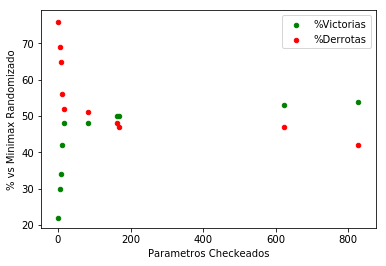
\includegraphics[width=0.4\textwidth]{GridBack.png}
	\caption{ Gráfico de \% victorias y \% derrotas en función de cantidad de parámetros checkeados por el Grid Search. Los porcentajes son sobre 100 partidos contra el minimax randomizado (50 empezando uno y 50 empezando el otro).}
\end{wrapfigure}


Se puede ver en la Figura 5 como efectivamente la cantidad de partidos ganados aumenta y la de partidos perdidos disminuye a lo largo que vamos checkeando más parametros. Se grafican solo los puntos donde cambia el actual campeon (en todos los intermedios se mantiene constante).

Con esta última modificación finalmente se obtuvieron los resultados esperados, comenzando con jugadores de valores aleatorios se veía un porcentaje de vicotorias bajo, pero a medida que se recorría la matriz de búsqueda se encontraban valores que obtenían mejores resultados a lo largo de las decenas de partidos contra el algoritmo óptimo. El descubrimiento de nuevos conjuntos de valores superiores al mejor hasta el momento ocurría con menos frecuencia (lo que se puede ver con claridad en la Figura 5 ya que los puntos cada vez estan más separados) pero esto es de esperar ya que el criterio de mejora es ahora mucho más exigente. Este nuevo criterio exigía una mejora real en la habilidad de un jugador dado, ya que lo enfrentaba a numerosas situaciones en las cuales debía jugar de forma razonable para poder vencer a este jugador óptimo, que era mucho más exigente que el aleatorio. 


Ahora sí cuando se observaba el comportamiento de los jugadores a medida que mejoraban su desempeño contra este criterio externo se podían ver respuestas razonables, obteniendo un porcentaje de 95\% de victorias frente a random, superior a los sorteados aleatoriamente que rondaban por el 91\% lo que se condice con la Figura 5 que muestra una clara mejoría respecto de la solución inicial.


\section{Algoritmo Genético}

El algoritmo genético se basa en la teoría genética darwiniana y busca básicamente recrear la evolución de una población. Los individuos más aptos tendrán mayor probabilidad de perdurar a lo largo de las generaciones, transmitiendo así los genes que hacen que sean más aptos. Se recrea también la mutación que permite que haya cambios en los genes (que pueden ser beneficiosos para la aptitud como no) de forma aleatoria. También se da el \textit{crossover}, donde los genes de uno de los individuos se cruza con los de otro, generando así nuevos individuos que no son copia de uno ni de otro sino una mezcla de ambos. Para mayor precisión, a continuación se encuentra el pseudocódigo. Solo hay que hacer una salvedad previa: para medir qué individuo es mejor que otro, se usaron dos funciones distintas de \textit{fitness}.

\subsubsection{El Pseudocódigo}
\begin{algorithm}
\SetKwInOut{Input}{Input}


    \Input{\textbf{int} rows, \textbf{int} columns, \textbf{int} c, \textbf{int} p}
 


\caption{genetico}

	\textbf{int} $tamanopoblacion$, $totalgeneraciones$

	\textbf{float} $min$, $max$, $pmutar$, $pcrossover$

	vector(conj(\textbf{parametro})) $poblacion$ = vector de longitud $tamanopoblacion$ donde cada elemento está dado por sendos llamados a \texttt{paramrandom}($c$)

	\For{$generacion = [1..totalgeneraciones$)}
		{

		poblacion = \texttt{seleccion}

		\For{$i \in poblacion$}
			{
			\texttt{mutar}($i$) con probabilidad $pmutar$
			}
		}

	\textbf{float} $maximo$ = \texttt{fitness}($poblacion[0]$, $poblacion$, $rows$, $columns$, $c$, $p$)

	\textbf{int} $maxpos$ = 0

	\For{\textbf{int} $i$ = [1..$poblacion$)}
		{

		\textbf{float} $actual$ = \texttt{fitness}($poblacion[i]$, $poblacion$, $rows$, $columns$, $c$, $p$)

		\If{$actual>maximo$}
			{

			actualizar $maxpos$ y $maximo$
			}
		}

	\textbf{return} $poblacion[maxpos]$

\end{algorithm}

Como muestra el pseudocódigo, el algoritmo lo que hace es establecer un tamaño de población e inicializa de alguna manera (en principio de forma aleatoria) a todos estos individuos. En nuestro caso, nuestros individuos son una estructura que contiene un valor particular para cada uno de los parámetros que tomaba la función del jugador parametrizable.

Hasta que se cumpla una condición de corte (en principio una cantidad fija de generaciones, pero esta variará siendo también un límite de tiempo, o podría ser también cierta condición de convergencia), se generarán nuevas poblaciones, que serán la próxima generación. Cada generación sufre un proceso de mutación y para dar lugar a una nueva, se da un proceso de selección que determina pares de individuos con los cuales se realizará el \texttt{crossover} dando lugar asi a un nuevo individuo que será parte de la próxima generación.

Para decidir a qué individuos seleccionar, se utiliza una función de \texttt{fitness} que basicamente decide (de alguna forma) cuán apto es un individuo. A partir de estos valores, el proceso de selección decidirá quiénes serán los que darán lugar a la nueva generación (en general, los más aptos son los que tienen más probabilidad de dar descendencia, ya que sus genes dan individuos más aptos).

A lo largo de toda la experimentación utilizamos diversas funciones de estas que se detallan a continuación.

\begin{itemize}
\item \textbf{\underline{Crossover:}} Consiste en, dados dos individuos (padres, dos estructuras de parámetros), generar un nuevo individuo que cada gen (cada parámetro particular) sea o bien de un padre o bien del otro. En nuestro caso toma un valor\textit{ pcrossover} que indica la probabilidad de que se cambie el padre del cual se están copiando los genes. El primer gen lo copia del primer padre pasado por parámetro, y cada vez que va al siguiente gen, sortea un numero (con una función random de distribución uniforme,\texttt{ rand()} de C++) en $[0,1]$. Si el resultado cae en $[0,pcrossover]$ copia el siguiente gen del otro padre. Sino sigue copiando del mismo. En principio, como los vectores que son parámetros (extensibles, extensiblesprox, biextensibles, consecutivos) presentan una clara relación entre ellos, decidimos que sean tomados como un gen entero (o bien se copia el vector de un padre o bien del otro)

\item \textbf{\underline{Mutación:}} Consiste en dado un individuo, cambiar cada uno de sus genes en base a alguna distribución de probabilidad. En nuestro caso, la función tomaba el valor\textit{ pmutar}. De forma análoga al\texttt{ crossover}, para cada gen se sorteaba un numero y si caía en $[0,pmutar]$ ese gen mutaba y pasaba a tomar un nuevo valor aleatorio entre un valor $min$ y $max$ que eran los valores mínimos y máximos que podía tomar el puntaje.


\item \textbf{\underline{Selección 1:}} Consiste en calcular el\texttt{ fitness} de todos los individuos de la población y para los que estén en una proporción de los que tienen más \texttt{fitness} (se fijo inicialmente en la mitad con más \texttt{fitness}) tomar dos aleatoriamente %(con distribución uniforme, usando rand() de C++ LO ESTAMOS DICIENDO TODO EL TIEMPO. CREERIA QUE YA SE SOBRENTIENDE, POR ESO LO SACO
) y a esos aplicarles \texttt{crossover} obteniendo así un individuo de la nueva población. Repetimos este proceso de tomar dos aleatoriamente de ese grupo hasta que la nueva población tenga el mismo tamaño que la anterior. Siempre se incluye tal cual estaba en la nueva generación al mejor de la anterior (esto se denomina elitismo, propiciamos que el mejor de todos se mantenga). Notar que si bien siempre se deja como estaba, este individuo (si no lo evitamos) podría sufrir alguna pequeña mutación.

\item \textbf{\underline{Selección 2:}} Consiste en generar grupos de un cierto tamaño (que se fijó inicialmente en el 20\% de la población) tomando a sus integrantes de toda la población (con distribución uniforme%, usando rand() de C++ IDEM ANTES
). Luego, dado un grupo se elegía al más apto dentro de ese grupo (al que tuviera mayor \texttt{fitness}), se repetía lo mismo obteniendo un segundo individuo (obtenido desde un nuevo grupo) y luego se realizaba \texttt{crossover} con estos dos obteniendo un individuo de la nueva generación. El proceso se repetía hasta que la nueva generación tuviera el mismo tamaño que la anterior. Nuevamente se utilizó elitismo, dejando en la nueva población tal cual estaba al mejor de la anterior.

\item \textbf{\underline{Fitness 1:}} Se hace jugar a cada individuo contra todos los de su población dos partidos, donde en uno empieza y en el otro va segundo. Se cuenta la cantidad de partidos en los que no perdió y se los divide por la cantidad de partidos jugados para normalizarlos (queda el \texttt{fitness} en [0,1] y además permite que quede en el mismo rango para disintos tamaños de población).


\item \textbf{\underline{Fitness 2:}} La idea de esta función de \texttt{fitness} es establecer un sistema de puntos. Nuevamente se hace jugar a cada individuo contra todos los de su población dos partidos, donde en uno empieza y en otro va segundo. Se da un puntaje según pierda, gane o empate (pierde$=0$; empata$=5$; gana$=10$) y se da un bonus si se empieza segundo ya que suponemos que en tableros medianamente grandes es una ventaja comenzar (BonusPierde$=1$; BonusEmpata$=2$; BonusGana$=4$). Luego, se divide al puntaje sobre la cantidad de partidos jugados (para poder tener los mismos valores de \texttt{fitness} en poblaciones de distintos tamaños).
\end{itemize}

Luego a lo largo de la experimentación se irán modificando estas funciones o agregando nuevas para ver la influencia de las mismas en el algoritmo.

\subsection{El algoritmo}



\subsection{Experimentacion}

Para comenzar con la experimentación, tratamos de comprender cómo influían los métodos de seleccion, funciones de\textit{ fitness, crossover} y\textit{ mutación} para así luego buscar la mejor forma de utilizar el algrotimo genético en nuestro caso. Para esto comenzamos estudiando estas funciones del algoritmo genético en el 4 en línea por ser una instancia particular que no es pequeña (tiene un tamaño considerable para ver diversas estrategias), ni es muy grande (los tiempos para experimentar son abarcables) pero podríamos haberlo hecho con cualquier otra sin problema.


\subsubsection{Funciones del Algoritmo Genético}

Primero, tratamos de comprender cómo afectaría el tamaño de las poblaciones. Si bien una población grande tiene como ventaja aportar mucha más variedad genética, los tiempos de ejecución son mucho mayores. Por su parte, una población pequeña si bien tiene poca variedad genética, es más eficiente en tiempo, dando muchísismas más generaciones en la misma cantidad de tiempo. Se buscó entender qué tipo de poblaciones brindaban mejores jugadores en el mismo tiempo. También se buscó encontrar qué\textit{ fitness} brindaba mejores jugadores y cómo eran las características de los métodos de selección.

Es por esto que se corrió el algoritmo genético para ambos métodos de selección y ambas funciones de \textit{ fitness} durante dos horas y media con poblaciones grandes, intermedias y chicas (de 100, 50 y 10 individuos cada una). Las poblaciones se inicializaron de forma aleatoria, donde cada parámetro se inicializaba aleatoriamente como un float entre -1 y 1 (con distribucion uniforme, se utilizo la funcion\texttt{ rand()} de C++). Las poblaciones de 100 individuos dieron 10 generaciones, las de 50 individuos dieron 37 y las de 10 individuos dieron 750 generaciones en el tiempo indicado. En todos estos casos, la probabilidad de mutar se fijo en 0.005 y la de $crossover$ en 0.4.




\begin{figure}[H]
	\captionsetup[subfigure]{position=b}
	\centering
	\subcaptionbox{tamaño 10}{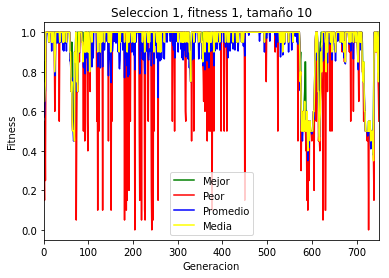
\includegraphics[width=0.3\linewidth]{s1f1t10.png}}
	\subcaptionbox{tamaño 50}	{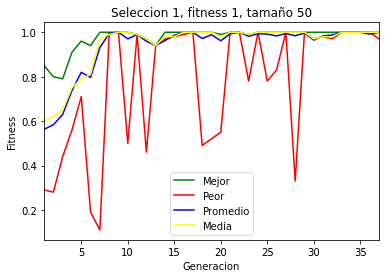
\includegraphics[width=0.3\linewidth]{s1f1t50.png}}
	\subcaptionbox{tamaño 100}{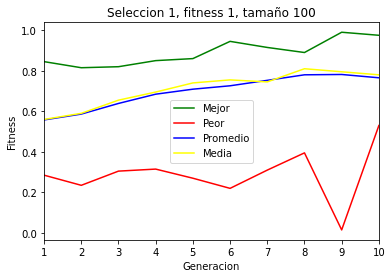
\includegraphics[width=0.3\linewidth]{s1f1t100.png}}
	\caption{Gráfico de \textit{fitness} en función de generación. Se grafica el mejor, peor, la media y el promedio. Selección 1, \textit{fitness} 1, $pmutar=0.005$, $pcrossover=0.4$}
\end{figure}

Como podemos observar en la figura 6, efectivamente a mayor tamaño de población, menor es la cantidad total de generaciones que se generan en el mismo tiempo (2.5 horas). Tanto en la Figura 6.a como la 6.b podemos ver que hay momentos en los que la población pareciera converger. O sea, el mejor, peor, promedio y media valen 1, que es el máximo valor de \textit{fitness} que pueden tomar (recordamos que estamos utilizando \textit{fitness} uno que es la proporción de partidos no perdidos sobre el total). En ambas, esta situación no se mantiene por el resto de las generaciones ya que hay mutaciones que perturban esta situación. Sin embargo es notable que en todos los casos la media sigue manteniéndose muy alta (casi 1, que es el valor máximo) a pesar de haber mutaciones (a excepción de la mutación que se ve en la Figura 6.a alrededor de la generación  100, 600 y 700). Además de la media, el mejor sigue también manteniéndose en valores máximos (a excepción de las mutaciones mencionadas). Esto puede suceder gracias al elitismo, puesto que aseguramos que el mejor individuo de la generación pasada se incluya en la nueva generación sin ser modificado. Si observamos los descensos de la media, no tienen un descenso del mejor (esto indicaría que se generan mutaciones que son peores individuos y desaparecen rápidamente, volviendo a converger) salvo en los casos señalados. Estas situaciones en las que cambia el mejor y la media, podrían ser en las que el mejor individuo muta. La otra opción sería que aparezca un nuevo individuo que es no es ni mejor ni peor que el que era el mejor hasta ahora. Es decir, a veces le gana y a veces pierde, por lo que ambos no tienen \textit{fitness} máximo. Esto último pareciera ser menos factible ya que no debería descender tanto la media por solamente un individuo así, a menos que sean varios, lo que es verdaderamente muy poco probable (ya es poco probable que varios muten considerablemente).

La convergencia de la media y el promedio a un valor cercano al máximo de \textit{fitness} pareciera ser rápida. En el caso de una población de tamaño 50 se da alrededor de la generación 10. En el caso de la de tamaño 10 se da tan solo en la quinta generación. Esto tiene sentido ya que es menor el tamaño de la población. Por último, en las 2.5 horas transcurridas, se ve un claro aumento de la media en la población de tamaño 100, pero no llegó aún a converger en dicho tiempo.

Más aún, cabe notar que una mutación en una población pequeña la afecta mucho más que en una población grande (porque es una cantidad de genes mucho mas significativa respecto del total). Estos gráficos ayudan claramente a reforzar dicha hipótesis. Esto se puede ver ya que las variaciones repentinas, a mayor tamaño de población son más suaves, ya que en el gráfico de la Figura 6.a hay ver picos muy acentuados en los que desciende hasta por debajo de 0.8, situación que en la Figura 6.b no desciende por debajo de 0.9 siquiera -una vez que ya convergió-. Más aún, si observamos la figura 6.c vemos que la media siempre aumenta, a excepción de la generación 7 donde disminuye casi despreciablemente. 

Cabe destacar que esta poca variabilidad que hay en la función de \textit{fitness} y la rápida convergencia se puede deber no solo a que se tratan por igual las victorias y empates, tanto se empiece o no, sino también a que el método de selección solamente toma los genes de los mejores individuos (de la mitad superior), por lo que la variabilidad es menor. Para tratar de comprender mejor esto, se realizó la misma experiencia con la funcion de \texttt{fitness2}, que distinguía empates de victorias y quién comenzaba.





\begin{figure}[H]
	\captionsetup[subfigure]{position=b}
	\centering
	\subcaptionbox{tamaño 10}{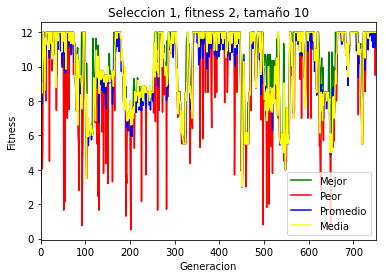
\includegraphics[width=0.3\linewidth]{s1f2t10.png}}
	\subcaptionbox{tamaño 50}	{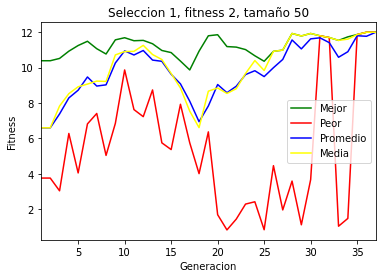
\includegraphics[width=0.3\linewidth]{s1f2t50.png}}
	\subcaptionbox{tamaño 100}{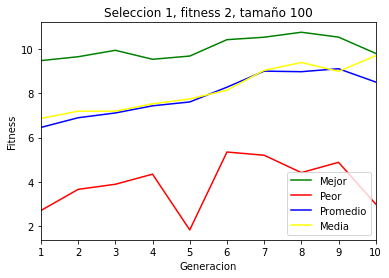
\includegraphics[width=0.3\linewidth]{s1f2t100.png}}
	\caption{Gráfico de \textit{fitness} en funcion de generación. Se gráfica el mejor, peor, la media y el promedio. Seleccion 1, fitness 2, $pmutar=0.005$, $pcrossover=0.4$}
\end{figure}

Efectivamente como podemos ver en la Figura 7, la variabilidad aumenta mucho más al cambiar la función de \textit{fitness} como esperabamos ya que esta distingue muchas más situaciones (distingue empates de victorias y distingue si uno empieza o no). Para todos los tamaños de población la media y promedio sufren alteraciones mayores en comparacion con la media y promedio de su gráfico análogo con la otra funcion de \textit{fitness}.

Algo destacable de esta función de \textit{fitness} es que las mutaciones y cambios en generaciones modifican el \textit{fitness} del mejor, que disminuye varias veces bastante (cosa que prácticamente no sucedia con la anterior función de \textit{fitness} -ver Figura 6-). Esto último sucede porque el \textit{fitness} depende mucho más del resto de los jugadores ya que considera más situaciones. Además, la convergencia sucede varias generaciones después que con la primer función de \textit{fitness} (en el caso de poblacion 50 se puede ver una convergencia recién en las últimas generaciones, las mayores a 30, mientras que con el otro \textit{fitness} era a la décima generación). 

Analizando el gráfico 6.a podemos ver que las mutaciones afectan mucho más al \textit{fitness} ya que la media desciende considerablemente, llegando a la mitad de su valor máximo en reiteradas ocasiones. Nuevamente podemos observar que las mutaciones afectan mucho más en poblaciones pequeñas, como se observaba en la Figura 6.

Teniendo entonces un análisis de la interacción entre la selección 1 con los dos \textit{fitness}, repetimos el análisis pero con la selección 2.



\begin{figure}[H]
	\captionsetup[subfigure]{position=b}
	\centering
	\subcaptionbox{tamaño 10}{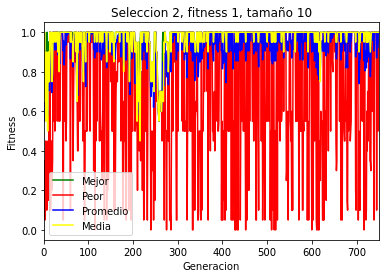
\includegraphics[width=0.3\linewidth]{s2f1t10.png}}
	\subcaptionbox{tamaño 50}	{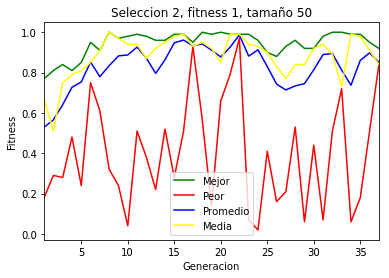
\includegraphics[width=0.3\linewidth]{s2f1t50.png}}
	\subcaptionbox{tamaño 100}{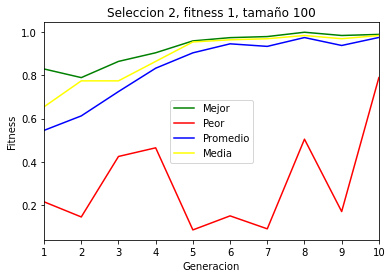
\includegraphics[width=0.3\linewidth]{s2f1t100.png}}
	\caption{Gráfico de \textit{fitness} en función de generación. Se grafica el mejor, peor, la media y el promedio. Selección 2, \textit{fitness} 1, $pmutar=0.005$, $pcrossover=0.4$}
\end{figure}


\begin{figure}[H]
	\captionsetup[subfigure]{position=b}
	\centering
	\subcaptionbox{tamaño 10}{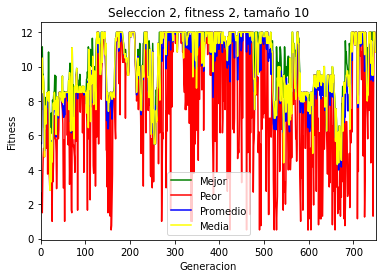
\includegraphics[width=0.3\linewidth]{s2f2t10.png}}
	\subcaptionbox{tamaño 50}	{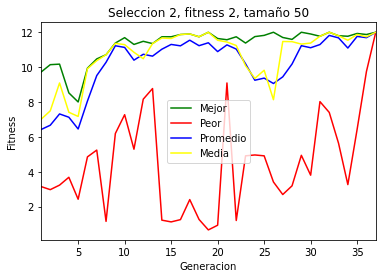
\includegraphics[width=0.3\linewidth]{s2f2t50.png}}
	\subcaptionbox{tamaño 100}{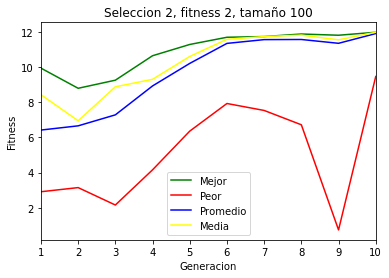
\includegraphics[width=0.3\linewidth]{s2f2t100.png}}
	\caption{Gráfico de \textit{fitness} en función de generación. Se grafica el mejor, peor, la media y el promedio. Seleccion 2, \textit{fitness} 2, $pmutar=0.005$, $ pcrossover=0.4$}
\end{figure}

En las Figuras 8 y 9 podemos ver características que refuerzan que ciertas situaciones se daban según lo conjeturado. Por ejemplo, nuevamente vemos que el \textit{fitness} 2 da mayor variabilidad y reduce más veces el \textit{fitness} del mejor. Nuevamente podemos ver también que la convergencia es más rápida con la función de \textit{fitness} 1, reforzando la hipótesis de que es porque esta considera menos situaciones (no distingue victoria de empate ni si empiezo o no).

Por último, una importante diferencia entre los gráficos con distintos métodos de selección es que los que usan el segundo método presentan peor caso con mucho menor \textit{fitness} y mucha más variabilidad (el desvío estandar es mucho mayor, lo que nos indica una convergencia que es mas lenta). Esto tiene sentido, ya que en el método de selección 1 solo se reproducían los que eran del 50 \% con mejor fitness, mientras que en el método de seleccion 2 se puede reproducir cualquiera de los que estén en el 80 \% de mejor \textit{fitness} (ya que el torneo era de tamaño del 20 \% de la población y el 20 \% peor nunca podría ganar alguno). En este sentido, la selección 2 si bien aporta más variabilidad, tiene peores jugadores.


Tras este análisis, tratamos de entender cómo afectaban las dos variables que quedaban por ver, que eran el porcentaje de mutación y el de $crossover$. Para ver cómo afectaba la probabilidad de mutación, ejecutamos con el primer método de selección, ya que es el que proveía menor variabilidad genética y perimtiría visualizar mejor cómo afecta el porcentaje de mutación. También se utilizo la primer función de \textit{fitness} por el mismo motivo. Por esto se ejecuto durante 5 horas, la población de tamaño 50 (intermedia, para tener una cantidad considerable tanto de generaciones como de individuos en la población) con diferentes probabilidades de mutar, con $pmutar=0.00001$, $0.005$, $0.01$, $0.05$ y $0.1$. El $crossover$ se fijó en $0.4$.


\begin{figure}[H]
	\captionsetup[subfigure]{position=b}
	\centering
	\subcaptionbox{pmutar 0.00001}{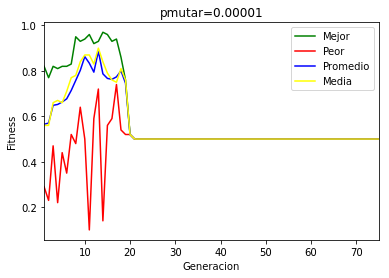
\includegraphics[width=0.3\linewidth]{muta0.png}}
	\subcaptionbox{pmutar 0.005}	{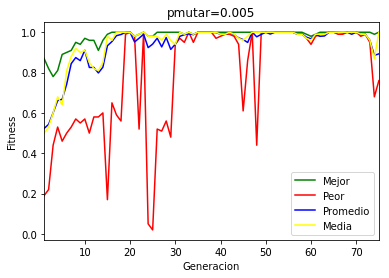
\includegraphics[width=0.3\linewidth]{muta1.png}}
	\subcaptionbox{pmutar 0.01}{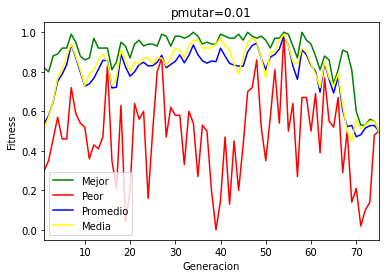
\includegraphics[width=0.3\linewidth]{muta2.png}}
	\subcaptionbox{pmutar 0.1}{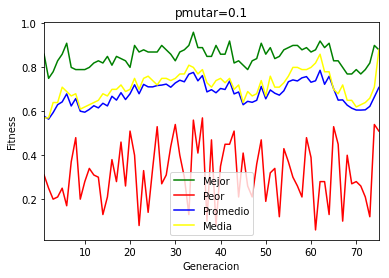
\includegraphics[width=0.3\linewidth]{muta3.png}}
	\caption{Gráfico de \textit{fitness} en función de generación. Se grafica el mejor, peor, la media y el promedio. Selección 1, \textit{fitness} 1, $pcrossover=0.4$}
\end{figure}

La Figura 10 refleja claramente lo esperado. En nuestro algoritmo genético hay operaciones que favorecen la convergencia, como es el proceso de selección y $crossover$, y hay en oposición operaciones que favorecen la divergencia, como es el caso de la mutación, lo que se puede ver claramente en esta Figura (figura 10). Con menores probabilidades de mutación, la convergencia no solo es más rápida, sino que los cambios en el \textit{fitness} una vez que convergió la población (momentos donde cambia la media) son cada vez menos. En la Figura 10.d podemos ver que hay bastantes picos, tanto en la media como en peores, mejores y promedio. Esto es porque la probabilidad de mutación es altísima (es un 10 \% para cada gen y hay 28 genes por individuo en este tablero) por ende es muy probable que todo individuo mute. En la Figura 10.c) la situación es la misma ya que un 1 \% para cada uno de los 28 genes sigue siendo bastante alto (cada individuo tiene un 25 \% de mutar que es es $1- (0.99)^{28}$ o sea, la probabilidad del complemento, que es que no haya mutación en ninguno de los 28 genes). En estas dos figuras no se llega a ver una convergencia en las generaciones que se dieron (podemos conjeturar que un porcentaje de mutación tan alto no va a permitir esta convergencia). Ya en la Figura 10.b podemos ver que hay efectivamente convergencia, pero como sigue habiendo un porcentaje considerable de mutación, hay generaciones donde se sale de este pico un poco (en algunas desciende un poco la media y el promedio, mientras que en otras solo desciende el peor). Finalmente en la Figura 10.a vemos una convergencia mucho mas rápida y una vez que esta se dio, todos los \textit{fitness} se mantienen así durante más de 50 generaciones. Esto es porque al poner una probabilidad tan baja, la mutación practicamente no sucede y no hay otras operaciones que permitan divergencia.

Por otro lado, la selección y el $crossover$ son operaciones que favorecen y buscan la convergencia. Para ver la influencia de la variable restante, el $pcrossover$, se ejecutó durante 5 horas, para la población de tamaño 50 (intermedia, para tener una cantidad considerable tanto de generaciones como de individuos en la población) con diferentes probabilidades de mutar, con $pcrossover= 0.4, 0.1, 0.01, 0.00001$.  El $pmutar$ se fijó en $0.005$.


\begin{figure}[H]
	\captionsetup[subfigure]{position=b}
	\centering
	\subcaptionbox{pcrossover 0.00001}{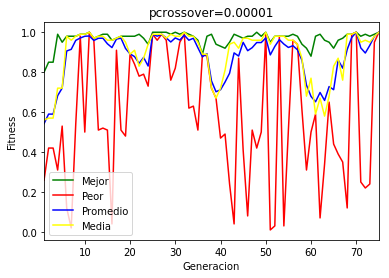
\includegraphics[width=0.3\linewidth]{crossover00.png}}
	\subcaptionbox{pcrossover 0.01}{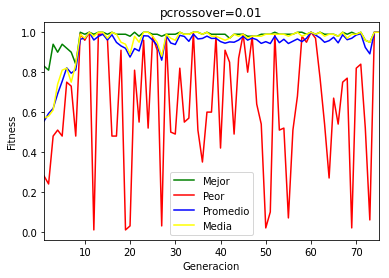
\includegraphics[width=0.3\linewidth]{crossover0.png}}
	\subcaptionbox{pcrossover 0.1}	{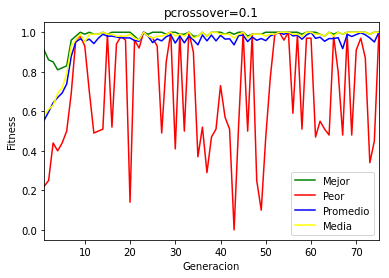
\includegraphics[width=0.3\linewidth]{crossover1.png}}
	\subcaptionbox{pcrossover 0.4}{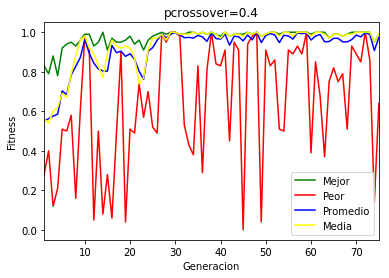
\includegraphics[width=0.3\linewidth]{crossover2.png}}
	\caption{Gráfico de fitness en funcion de generación. Se gráfica el mejor, peor, la media y el promedio. Seleccion 1, fitness 1, pmutar=0.005}
\end{figure}

Como podemos ver en la Figura 11, en contra de lo esperado, pareciera no haber una convergencia más rápida si aumentamos $pcrossover$. Sin embargo, considerando que la probabilidad es para cada uno de los genes, la probabilidad de $crossover$ de $0.4$ resulta altísima (considerando que para esta instancia de tablero particular hay 28 parametros), por lo que los individuos mezclan demasiado sus genes, tardando mucho más en converger que en el resto. Por otra parte, reforzando la hipótesis de que favorece la convergencia, si vemos algo con $pcrossover$ realmente bajo como es el caso de $0.00001$ en comparación con $0.01$ la convergencia es más lenta una vez que se sale de esta (la media desciende mucho más y tarda más en tomar nuevamente el valor de convergencia).

Quizás algo que pueda estar influyendo es que primeramente decidimos dejar a los vectores como una unidad, como todo un gen que se transmitía o bien de un padre o del otro. Por ende, realizamos la misma experiencia solo que ahora se decidía de qué padre copiar cada uno de los elementos del vector según $pcrossover$, o sea, con este cambio el hijo puede tener una parte de un vector de uno y la otra parte del otro.

\begin{figure}[H]
	\captionsetup[subfigure]{position=b}
	\centering
	\subcaptionbox{pcrossover 0.00001}{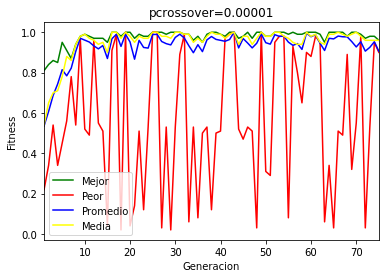
\includegraphics[width=0.3\linewidth]{crossoverB00.png}}
	\subcaptionbox{pcrossover 0.01}{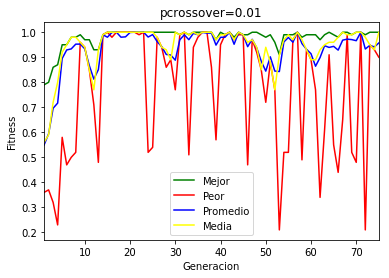
\includegraphics[width=0.3\linewidth]{crossoverB0.png}}
	\subcaptionbox{pcrossover 0.1}	{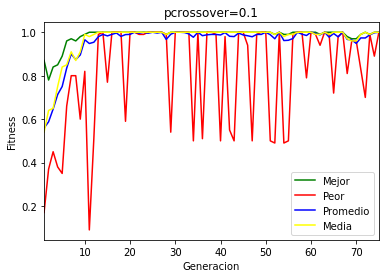
\includegraphics[width=0.3\linewidth]{crossoverB1.png}}
	\subcaptionbox{pcrossover 0.4}{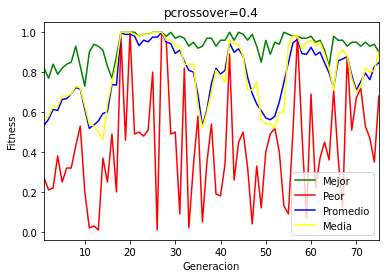
\includegraphics[width=0.3\linewidth]{crossoverB2.png}}
	\caption{Gráfico de \textit{fitness} en funcion de generación. Se grafica el mejor, peor, la media y el promedio. Selección 1, \textit{fitness} 1, $pmutar=0.005$}
\end{figure}

Este cambio no pareciera sin embargo reflejar algo muy distinto, la única diferencia es que aporta un poco más de variabilidad en todos los casos, lo que se puede notar claramente en el gráfico 11.d ya que la media y promedio presentan mayores cambios en comparación con el gráfico 10.d, no presentan una convergencia sostenida en varias generaciones (ni siquiera en 11). Es esperable que aporte más variabilidad debido a que los individuos mezclan sus genes mucho más, dando lugares a nuevas posibilidades de valores de los vectores que son parámetro, cosa que antes solo se daba con mutaciones eventuales.

Sin embargo, con este cambio también, podemos notar que no hay influencia en la velocidad de convergencia por parte de la probabilidad de $crossover$, contrariamente a como esperabamos que sea al principio. Esto podría ser debido a que los parámetros, al ser la importancia de cada cosa, son bastante independientes entre sí y no tenemos bloques grandes que estén correlacionados entre sí en cuanto al juego (a lo sumo los pares que determinan mi importancia respecto de la del otro), por lo que no es tan relevante si copiamos toda una tira de parámetros de un mismo padre. Esta idea surge al ver que no pareciera haber cambios en la velocidad de convergencia cuando rompimos esas tiras (lo que graficamos en la Figura 12).

Sí, en cambio, resulta importante para dar más variabilidad y evitar que la media se quede en valores cercanos al de convergencia como claramente se puede ver que sucedió en el gráfico de la Figura 12.d, donde además de ser alta la $pcrossover$, usamos la segunda forma donde miramos como gen heredable de algún padre a cada elemento del vector y no a este en su totalidad.

\subsubsection{Jugadores}
Habiendo estudiado entonces la influencia de los distintos parámetros, tratamos de buscar una combinación de estos que dé un buen jugador. Todos los jugadores que fueron generados al final (el mejor de la última generación para cada experimento) compitieron entre ellos.

En los primeros experimentos con 2.5 horas, para cada función de \textit{fitness} y cada método de selección, hicimos competir a los tres jugadores todos contra todos dos partidos, donde se alternaba quien comenzaba. Para el método de selección 1, con ambas funciones de \textit{fitness} resultaron ganadores siempre los segundos jugadores y después se vió que jugaban prácticamente partidos similares donde jugaban en las casillas de más cercanas al borde. Como reflejaban los parámetros, se le daba lo que pareciera ser poca importancia a los biextensibles y extensibles en general. Al jugarle a estos jugadores, todos perdieron rápidamente ya que ninguno tomaba el centro, y al armar rápidamente una linea de 2 que sea biextensible, como no era cubierta, pasaba a ser una de tres biextensible, lo que sentenciaba la derrota del programa. Aquí no se pudo ver diferencia entre las tres poblaciones a simple vista ya que eran malos jugadores los tres. Pero con el método de selección 2 el panorama fue distinto...

Primero, con la función de \textit{fitness} 1, el jugador de población inicial de tamaño 100 resultó ser el peor (perdía o empataba, según empezara o no). Luego, los de tamaño 50 y 10 quedaron empatados (ganaba el segundo). Esto nos refuerza nuestra hipótesis de que la poca evolución que presentó el de población de tamaño 100 (tan solo 10 generaciones) no permitió que se desarrollen buenos individuos. Luego le jugamos a cada uno de estos dos y resulto que el de tamaño 10 no detectaba biextensibles (al igual que cuando usabamos selección 1) pero el de tamaño 50 sí logró detectar biextensibles, jugando mucho mejor que el de 10 y perdiendo porque no pude detectar una linea que era extensible en el próximo turno de tamaño $c-1$. Esto refuerza la hipótesis de que tener una población de tamaño 10, si bien evolucionaba mucho (dando 750 generaciones) tenía tan poca variabilidad que daba malos jugadores. Más aún, tiene sentido que sean peores porque en la función de \textit{fitness} (en ambas) evaluó los partidos contra todos los de su generación, por lo que al ser pequeña la población, se jugaban menos partidos y con mas fácilidad se obtenía un \textit{fitness} alto (esta es una clara diferencia respecto del paper, en la que se ahondará más adelante). 

Más aún, con el método de selección 2 y la función de \textit{fitness} 2, el jugador de la población de tamaño 10 fue el peor del torneo, perdiendo todos los partidos, lo que refuerza nuestra idea. Como vimos, este método y este \textit{fitness} eran los que presentaban mayor variabilidad, pero al tener una población esto se desaprovechaba, lo que indicaría el motivo de por qué la de tamaño 10 perdió todos los partidos. Luego, la de tamaño 50 ganó todos los partidos, siendo la mejor de las tres. Esto refuerza más aún nuestra hipótesis de que no conviene una población muy grande ya que permite poca evolución (pocas generaciones) ni una tan pequeña ya que da poca variabilidad; la de tamaño intermedio (50) permite tener tanto una variabilidad como una evolución considerables. Nuevamente, para ver las estrategias y cuán bueno era cada uno, les jugamos nosotros y el de 100 no tomó el centro ni detectó biextensibles por lo que perdió rápidamente. En el caso del de 10, sucedió lo mismo. Sin embargo, en el caso del de 50, tomo el centro, cubrió extensibles nuestros, no permitió que generáramos biextensibles (quizás no los detecta, pero por lo menos no lo permitió) y terminó ganando ya que hubo un momento que ambos jugadores llenamos el tablero por no poder jugar en una columna ya que ganaría el otro. Repetimos varios juegos contra este jugador, empezando nostros y notamos que cubría biextensibles al principio del juego, pero avanzado el juego dejaba de hacerlo y perdía por eso. Efectivamente, observando los parámetros podemos ver que le da importancia biextensibles (más a generarlos que evitar que el otro lo haga) y a los extensibles en la próxima (más a taparlos que generarlos), pero no es mucho mayor que otras comparativamente por lo que al haber más características en juego, podría dejarlos de lado. Le daba importancia a jugar en el centro también.

Esta experimentación nos permitió ver que resultaba más efectivo, en la misma cantidad de tiempo, una población de tamaño intermedio (50) que una chica (10) o grande (100) ya que proveía tanto evolución como variabilidad genética. Más aún nos mostró que los métodos de \textit{fitness} cobraban más importancia al tener una población mayor (ya que se completan más partidos). También nos mostró que dio mejores resultados el proceso de selección 2, lo que tenía sentido ya que aportaba muchísima más variabilidad genética. Dentro del proceso de selección 2 se noto claramente que daba mejores resultados una población intermedia y también que la función de \textit{fitness} 2 era más efectiva (ya que diferenciaba más situaciones, que al jugar partidos solo contra los de nuestra generacion, se volvían importantes estas diferencias) puesto que aportaba más variabilidad.

Por estos resultados y todo lo analizado, decidimos a la hora de buscar jugadores buenos utilizar el proceso de selección 2, la funcion de \textit{fitness} 2 ya que aportan más variabilidad y distinguen más situaciones. Tomamos una población de tamaño 50 que daba una variabilidad considerable y también permitía realizar varias generaciones sin tomar tanto tiempo, además porque este tamaño daba más fidelidad a la función de \textit{fitness} ya que para determinar cuan bueno era un jugador lo hacíamos competir contra más rivales. La probabilidad de $crossover$ la fijamos en $0.4$, y tomamos cada elemento de los vectores como un gen, para asegurar que haya variaciones dentro de los parámetros que utilizan ya los jugadores seleccionados. La probabilidad de mutar se fijó en $0.005$ para asegurar que haya variaciones pero no sean demasiadas como para evitar la convergencia.

Se ejecutó esto durante 10 horas (en un total de 150 generaciones) y se obtuvo así un jugador que parecía ser bastante bueno y superador (le ganaba al obtenido anteriormente con una población de tamaño 50 y dos horas, lo que tenía sentido pues se entrenó durante más generaciones). Como un primer chequeo de la validez de este método y que efectivamente se trataba de un jugador con una estrategia definida, se lo hizo competir 1000 veces contra el jugador random siendo segundo y perdió 49 veces, empataron 2 veces y siendo primero perdió 21 veces y empataron 2 veces. Si consideramos los 2000 partidos jugados, no ganó solo 74 veces, o sea que ganó en un 96,3 \% de los partidos (efectivamente mayor a cuando se ponían parámetros aleatorios). Esto valida que nuestro jugador era bueno, considerando que salió de una población incial en que todos los valores eran aleatorios. Más aún, creamos un jugador nosotros con parámetros puestos a mano que creíamos que serían los mejores y ese jugador perdió contra el que la máquina había dado, tanto siendo primero como segundo, aunque obtuvo mejores resultados contra el random (ganó en un 100 \%).


Sin embargo, algo de mucha importancia no analizado aún es que como solo competimos dentro de los jugadores de nuestra generaciones, sería bueno tener jugadores bastante variados, con diversas estrategias y que le den mas importancia a algunas características que a otras. Si bien, como ya se dijo, obtuvimos un jugador bueno en la experimentación hasta ahora realizada, no era lo suficientemente bueno (no superaba en principio al que nosotros le elegimos los parametros). Por esto, decidimos para ver si obteníamos mejores jugadores, brindar una población con alguna estrategia inicial buena. Utilizamos entonces el jugador que propusimos que priorizara lo que creíamos era bueno (dar más importancia a biextensibles, extensiblesproximo, extensibles, jugar en el centro al principio) y al resto de la población la pusimos como random. Esto era factible de funcionar porque nuestra selección tiene elitismo, o sea que el mejor individuo anterior siempre es copiado tal cual, por lo que si nuestro jugador fuese el mejor, nunca debería ser reemplazado si nadie lo supera. Sin embargo, el mejor individuo seguía siendo factible de sufrir mutaciones, por lo que corrimos un caso donde el mejor individuo de la generación pasada no podía mutar. Se esperaba entonces que el jugador obtenido sea mejor que el inicial. Se ejecutó durante 10 horas (4 veces más de lo que se había dejado anteriormente), o sea un total de 150 generaciones. 

Tras esto, obtuvimos un jugador que resultó ser peor que nuestro jugador inicial (aunque no considerablemente peor, ganaba en un 98.6\% al random mientras que el inicial en un 100\% -sobre una muestra de 1000 partidos como primero y 1000 como segundo-). Si bien esto contraria lo esperado, podría ser debido algo similar a lo que sucede en\texttt{ grid search} cuando dimos una solución inicial a partir de la cual explorar el espacio, ya que al jugar solo partidos contra los de nuestra población (que además son todos determinísticos en cuanto a sus jugadas, dos jugadores -una vez fijado quién empieza- siempre jugarán el mismo partido) es bastante probable encontrar jugadores que sean ''malos'' en general pero que en particular le ganen a nuestro jugador ya que la rama de partido que se da entre ellos dos hace que gane el que es peor. De esta forma, no es raro que se genere un individuo parecido al inicial que le gane a este y pase a ser el nuevo de mejor \textit{fitness} pero que sea peor. De hecho, si bien empeoró, al ser mucho mayor la población en comparación con el primer metodo del grid search (jugamos contra 50 en vez de contra solo uno), el jugador empeoró mucho menos (redujo en 1.4 su porcentaje de victorias al random, mucho menos que en el grid). Esto es porque al tener una poblacion de 50 individuos, si bien deterministicos, chequeamos varias lineas de juego de cada jugador (como si jugaramos contra 50 individuos distintos).


Se repitió la misma experimentación en otro tablero con $N=9$, $M=8$, $C=5$ y $p=100$ (fichas de sobra). Donde, en cuanto a la distribución que determinaban los métodos de selección \textit{fitness} y $pmutar$ fue análoga, sin aportar mucha diferencia (como era esperable). Lo único que destacamos es que el pocentaje que le ganaba al random creció considerablemente (llegó a un 98.4 \% contra el 96.3 \%) en el obtenido por el algoritmo genético con una población inicial aleatoria. Esto lo atribuimos a que al ser mayor el tablero, es más difícil que el random gane ya que la probabilidad de caer justo en un juego en el que pierda (o que gane el random análogamente) es mucho menor porque hay más columnas donde jugar y es menos probable que el random haga algo bueno (en principio logre formar líneas). Además el $c$ es mayor por lo que para que el random gane debe alinear 5 fichas que es menos probable que 4. Efectivamente los resultados de la técnica pueden variar para distintos tableros, donde hay que tener en cuenta también que utilizar al jugador random para validar cada vez se vuelve menos viable al aumentar el tamaño del tablero. Para reforzar esto se repitió lo mismo con un tablero de $N=14$, $M=12$, $C=10$ y $p=500$ (fichas de sobra) y el jugador obtenido ganó en un 99.8\% de las veces.


Si bien utilizar al jugador random como una medida de fitness externa no tendría sentido por los mismos motivos que en grid (inicialmente el porcentaje de victorias ya es muy alto), sería bueno buscar alguna forma externa a la población actual de medir el fitness. Este podría ser un jugador externo que no sea determinista (pues sino sucederia lo mismo que en el grid al enfrentar a dos jugadores solo). Por esto se buscó alguna medida de fitness distinta que sea externa y permita medir de otra forma cuan bueno era un jugador dentro de la población, buscando mejores resultados. Intuitivamente, tomar medidas externas reflejaría mejor cuan bueno es un jugador ya que evitaría que todos los individuos tengan estrategias similares (ya que no importa sólo los resultados que obtienen entre ellos). Más aún si estas medidas fueran contra jugadores no deterministas permitirían detectar mas líneas de juego de nuestro jugador (si repitieramos el partido). 

Por esto se corrió (nuevamente en el 4 en línea) el algoritmo genético con una modificación en el fitness 2, donde en vez de jugar todos contra todos, jugaba cada uno 50 veces (25 empezando uno y 25 empezando el otro) contra el jugador minimax randomizado (que miraba cuatro jugadas a futuro, el mismo que se utilizó en grid search). Se lo dejo correr durante 20 horas. A continuación, graficamos en la figura 13 los resultados de este experimento

\begin{wrapfigure}{R}{0.4\textwidth}
	%\centering
	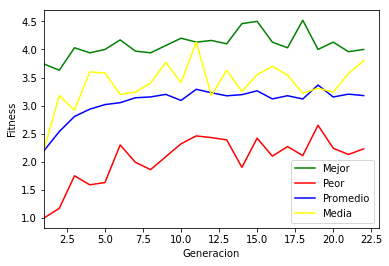
\includegraphics[width=0.4\textwidth]{GenBack.png}
	\caption{ Gráfico de \textit{fitness} en función de generación. Se grafica el mejor, peor, la media y el promedio. Se utilizó el fitness 2 modificado, donde se jugaba contra el minimax randomizado.}
\end{wrapfigure}

Antes que nada es destacable como al jugar contra el jugador minimax randomizado el tiempo de ejecución es mucho mayor, por lo que hay menos generaciones obtenidas en las 20 horas (mientras que con 10 horas obteniamos 150 generaciones con este mismo tamaño de poblacion y cantidad de partidos -solo que entre ellos y no contra minimax randomizado-). Podemos ver que al ser un fitness externo no suceden cambios tan abruptos en la media y en el promedio. Más aún, la convergencia es mucho más lenta (el jugador contra el que se entrena es bueno, se tarda mas en lograr un buen fitness). Efectivamente  podemos ver, como se espera, que el fitness va creciendo en líneas generales (y por ende los resultados que obtienen por sobre el minimax randomizado ya que así lo definimos) pero no es un crecimiento estricto (como lo era en grid search) lo que tiene sentido a causa de las mutaciones.

Efectivamente este resultado dió un mejor resultado contra el jugador random ya que le gano un 97.2 \% al jugador random, lo que fue superior al 96,3 \% obtenido con el fitness 2 inicial (sin minimax randomizado). Esto tiene sentido ya que se entrenaba viendo diversas lineas de juego por lo randomizado del minimax, sin embargo la diferencia no es tan marcada (como sí lo era en grid search) ya que en el otro caso se ven también varias lineas de juego ya que se juegan 50 partidos (todos contra todos dentro de la generación).



\section{Análisis comparativo con paper}

En comparación con el paper, antes que nada cabe destacar que hay grandes diferencias en los juegos. Si bien ambos son de dos jugadores, en el Tatetí la cantidad de configuraciones es abarcable (de hecho, sacando los no factibles y vía isomorfismos, los autores muestran que hay tan solo 827 configuraciones posibles) mientras que en el $c$ en línea esto no sucede por varios motivos. Primero que nada, como podemos variar el tamaño del tablero, la cantidad de configuraciones puede aumentar muchísimo y como la grilla (salvo contados casos) es mucho mayor, la cantidad de partidas que se pueden dar es mucho mayor ya que si miramos los tableros -factibles o no- el tatetí presenta $3^9$ y el $c$ en linea $3^{NM}$ donde $N*M$ suele ser mayor que 9 salvo contados casos. Como esta cantidad crece exponencialmente, al aumentar un poco $N$ y $M$, esta cantidad se hace inabarcable por lo que resulta imposible realizar una estrategia similar a la del paper (que mira la configuracion actual y para esa tiene definida que jugada hacer previamente en un arreglo).

Sin embargo, podemos adaptar la estrategia a nuestro juego particular y es por esto que se estableció un sistema de puntos que permitía caracterizar los posibles tableros que se pueden dar tras nuestra jugada y así elegir el que sea el mejor. Y es aquí donde entra la libertad que le damos al jugador para que luego trabaje el algoritmo genético. Esta libertad también existía en el paper y era mucho más flexible aún. De hecho era lo más flexible posible porque dejaba elegir para cada situación que jugar al algoritmo. En cambio, por la dimensión del problema, nosotros no podíamos dar tanta flexibilidad ya que resultaría inabarcable; por esto surge el sistema de puntos, nosotros tomamos ciertas características del tablero y permitimos que luego el algoritmo genético decida la importancia de cada una de esas características y juegue en base a dicha importancia. La función que establecía el puntaje de un tablero es la que en realidad toma los parámetros que el genético busco modificar y de hecho, estos parámetros son los que determinan la importancia de cada una de las características que nosotros decidimos. Aquí está la flexibilidad que tiene nuestro jugador (en algún punto, no es tan flexible ya que solo puede variar dentro de la importancia de las características que nosotros determinamos, todas las que no hayamos elegido no las podra distinguir).

Más aún, hay una notable diferencia que es que al ser menos flexible y tener que elegir qué características uno quiere que distinga el jugador para que luego el genético decida su importancia, pareciera ser muy importante la elección de estas características. Efectivamente lo es, pero nos permite ver algo que no sucedía en el paper, que es que poner características de más que no sean relevantes no es algo tan problemático ya que el algoritmo genético luego determinará que son poco o nada importantes. 

Además, nosotros tomamos dos funciones de \textit{fitness} que en esencia eran las mismas que en el paper para poder analizar cómo esto variaba según el juego. Efectivamente en nuestro juego, el c en línea, pudimos ver que el \textit{fitness} de puntaje fue más fructífero que el de proporción de partidos no perdidos. Nuestra hipótesis es que esto sucedió porque distinguía más situaciones (empate de victoria y empezar o ir último). Sin embargo, el hecho de que en el paper el sistema de punteos también distinguía más situaciones y haya resultado peor no contradice esto ya que hay una diferencia esencial en el cálculo de \textit{fitness} en ambos casos: nuevamente al ser una cantidad abarcable todos los tableros del ta-te-ti en el paper a un jugador se lo hace jugar todos los juegos posibles y se evalúa ahí cuántos no perdió y al ver todas las situaciones es claro que cobra mucha más importancia minimizar las perdidas. Mientras que en el c en línea resulta inabarcable hacer jugar a cada jugador de cada generación todos los partidos posibles (ya hacer jugar a un jugador todos los partidos posibles es caro como la primer jugada de\texttt{ minimax}, que en tableros grandes puede tardar muchísimo tiempo en jugar por el crecimiento exponencial que presenta esta cantidad), por lo que importa mucho más tener en cuenta estas diversas situaciones ya que la cantidad de partidos que podemos hacer jugar a un jugador es mucho más acotada.

Incluso esto nos permitió entender por qué no tuvieron éxito las poblaciones de 10 jugadores ya que ademas de presentar una poca variabilidad, las funciones de \textit{fitness} se basaban en partidos contra muy pocos jugadores. En este caso, a diferencia del paper, variar los tamaños de las poblaciones sí mostró mejoras en los jugadores (no lo hizo en el \textit{fitness} final del mejor jugador de la última generación). Por el tamaño del problema, nuevamente, resulta imposible encontrar un jugador óptimo, cosa que fue posible por medio del algoritmo genético en un problema más pequeño como es el del tatetí. Lo que sin embargo se busco hacer es encontrar un buen jugador de c en línea a través de encontrar los parámetros adecuados para el jugador parametrizable por medio del algoritmo genético.

Esto último va de la mano con lo que miden las funciones de \textit{fitness}, ya que en el c en línea no fue posible definir una función que midiera realmente cuán bueno era un jugador ya que eso implicaría jugar todos los partidos posibles lo que no era abarcable. Sí permitían ver cuán bueno era un jugador comparativamente en relación con otro/s (lo que se determinaba simplemente haciendolos competir). Por esto, nuestro algoritmo genético con estas funciones de \textit{fitness} podía dar buenos jugadores pero no óptimos, ya que requeriría en principio alguna medida de cuán bueno es un jugador en todas las situaciones. Más aún se pudo ver como afecto en la calidad de jugadores establecer mejores formas de determinar cuan bueno era un jugador (jugando uno contra uno en el grid, luego jugando todos contra todos en una misma generacion del genético, jugando reiteradas veces contra el random o contra el minimax randomizado que miraba 4 jugadas adelante). Esta situación no se dió en el paper con el tatetí ya que era clara la forma de determinar cuan bueno era un jugador, por lo pequeño del problema (era abarcable jugar todos los partidos posibles).

\section{Conclusiones}

Concluimos primeramente que presentamos un jugador óptimo mediante la técnica de\textit{ minimax}, que salvo para tableros muy pequeños, era inviable ya que consideraba todas las posibilidades de juegos que se podían dar y tomaba en las que se maximizaba el resultado (considerando que el otro jugador quería minimizar dicho resultado -el resultado es gano yo, empatamos o perdemos, con ese orden por lo que maximizar es buscar ganar, cosa que si no se puede empatar y si tampoco se puede, perder; recíprocamente es minizar-). Se mostró que este algoritmo hacía cada jugada en $\mathcal{O}(N\textsuperscript{((N+1)M)+1})$ (se mostró una mejor cota que implicaba las casillas libres en el momento y las columnas donde se podía jugar, lo que se acotó por esta complejidad). Por ser de un gran tiempo de ejecución, se dio el mismo algoritmo con la poda $\alpha - \beta$ que concluimos permitió ejecutar el algoritmo en menor tiempo, pero para tableros que no sean pequeños seguía siendo inviable ya que el tiempo de ejecución seguía siendo altísimo porque si bien no se analizaba todo el árbol de minimax, si se chequeaba una gran parte del mismo. La poda si bien se ejecutaba, no nos permitía asegurar una complejidad teórica menor, aunque sí un menor tiempo de ejecución que se comprobó experimentalmente.

Teniendo esto en cuenta, se busco generar un jugador que tenga un tiempo de ejecución considerable jugada a jugada y que analice sólo una jugada adelante (no más, ya que sino sería como hacer -al menos por unas jugadas- minimax). Este jugador era goloso en el sentido de que decidía la mejor de las siguientes jugadas (en nuestro caso la que de un tablero de mayor puntaje). La idea era que este jugador tenga parámetros que se dejen libres, para despues buscar qué valores tenían que tomar para dar un mejor jugador. Se mostró experimentalmente que este jugador tardaba $\mathcal{O}(N^2M)$ en realizar cada jugada. Estos parámetros que se dejaron libres fueron características del juego decidida por nosotros y luego se mejoraría al jugador decidiendo qué características eran más importantes. Este trabajo se hizo con dos técnicas distintas:\texttt{ Grid Search} y un Algoritmo Genético.

De la experimentación con la heurística \texttt{ Grid Search} la principal conclusión es la importancia de la selección del mejor jugador entre 2 candidatos. Es de esencial importancia, y de hecho sin esto fallaron los primeros intentos del \texttt{ Grid Search}, una función que pueda valorar la flexibilidad de un jugador frente a distintas situaciones, ya que sin esto es muy fácil caer en un jugador muy bueno para ciertas situaciones pero desastroso frente a un jugador que presente distintas lineas de juego. Es importante en el comienzo de cualquier proyecto que implique \textit{machine learning} el diseño de un método de evaluación para los parametros que sea no sólo exigente, si no abarcativo, para asegurarse el aumento de la eficiencia en múltiples situaciones. Basicamente es fundamental dar una forma de decidir que cosa es mejor que otra (o más apta) que responda a lo que estamos buscando. En nuestro caso, comparar tan solo dos jugadores entre sí abarcaba muy pocas situaciones (solo dos líneas de juego de todas las que tiene un jugador), jugar contra random resultaba muy simple (ya que al ya haber destacado ciertas características relevantes al juego, por malo que sean los parámetros se le ganaba facilmente) fueron de malos resultados. Los resultados mejoraron claramente al decidir que un jugador era mejor que otro por medio de muchas iteraciones contra un jugador minimax randomizado que veía 4 jugadas adelante.

Las numerosas iteraciones del algoritmo genético con distintos tamaños poblacionales y parametros para las mutaciones, crossover y distintos métodos de fitness y selección nos permiten concluir que se debe buscar un tamaño de población medio que sea lo suficientemente pequeña como para correr numerosas generaciones, pero que además permita suficiente variabilidad genética, por dos razones. La variabilidad genética es importante no sólo a la hora del crossover para la nueva generación, si no que debe permitir distintas estrategias, que no converjan rápidamente a una sola forma de juego, para así asegurar que al enfrentar a todos los jugadores entre sí se están explorando efectivamente distintas líneas de juego, de lo contrario se caería en una situación similar a la experimentada en el \texttt{ Grid Search}.

Se reconoció también la importancia de utilizar métodos de fitness que distingan entre múltiples situaciones, empezando el partido el jugador a evaluar o sus oponentes, distinguiendo entre un jugador que siempre gana, siempre empata o siempre pierde, por ejemplo. Más importancia cobra distinguir situaciones como quien empieza (no solo si se pierde, gana o empata) cuando no es posible ver todas las situaciones posibles del juego (cosa que si era factible en el paper, por lo que se utilizo un fitness que no distinguía mas que si se perdía o no). Por esto concluimos que se obtuvieron mejores resultados con el fitness 2 que con el fitness 1. El método de selección debería por una parte favorecer aquellos jugadores con un fitness mayor, pero siempre dando una oportunidad a aquellos no tan buenos para mantener suficiente variabilidad genética, dando lugar a explorar nuevas características de jugadores (en donde luego actuará la selección en base al fitness para decidir si estas prosperarán o no). Esto se condice con que el metodo de selección 2 dió mejores jugadores que el método de selección 1. Se vió también la importancia de la mutación en el proceso del algoritmo genético, siendo necesaria para asegurar diversos individuos y dar variabilidad (lugar a nuevos individuos con estrategias diversas que la selección decidirá si perdurarán o no), pero que no sea muy alta para asegurar la eventual convergencia de la población. En cuanto al crossover, se concluyó que no era tan influyente la probabilidad que se tomara en este algoritmo genético particular.

Como resumen, se destacan dos cosas necesarias para poder observar una verdadera mejora en el jugador por medio de las heurísticas estudiadas. En primer lugar es necesaria la exploración del espacio de búsqueda, probar variados conjuntos de valores, ya que sin esta exploración hay opciones que uno nunca considera. En el \texttt{ Grid Search} esto se podía ver en la prueba de mover todos los parametros con valores a lo largo de todo el rango [-1,1], y si bien no se exploraba todo el espacio esto se debe a la imposibilidad de esa tarea. En el algoritmo genético la exploración del espacio se realiza de mejor forma con una mayor variabilidad genética que evita el estancamiento en un vecindario de soluciones reducido, por esto resultaba tan importante el uso del método de fitness y de selección 2. En particular, el algoritmo genético es una heurística que nos permite no solo encontrar buenas soluciones, sino no quedarnos al rededor maximos locales (gracias a las mutaciones) y explorar el espacio en general.

El segundo requisito esencial es que la función con la cual se califica la habilidad de un jugador refleje fielmente esto. La misma debe contemplar múltiples y variados casos a los cuales la función parametrizable debe responder, ya que de lo contrario los jugadores optimizados no mostraran un buen desempeño frente a las amplias situaciones a los que deben saber enfrentarse (ya que solo analizarán contadas lineas de juego, mientras que tienen tantas como configuraciones un tablero). Es necesario que presenten varias situaciones (no solo mirar pocos partidos en particular) para poder captar la esencia de la estrategia de cada jugador.

 Es difícil en un problema de muchas configuraciones posibles como es el c-en línea establecer qué significa que un jugador sea mejor que otro o cuán bueno es un jugador. En cuanto a esto, vimos la poca efectividad de enfrentar dos jugadores entre sí ya que solo exploraban dos líneas de juego de toda su estrategia y podría tranquilamente un jugador muy malo ganarle a uno muy bueno en esa partida en particular. Esto, al aumentar la cantidad de gente que jugaba entre sí mejoró considerablemente como se vio en el algoritmo genético donde $50$ individuos jugaban todos contra todos. También es deseable tener algún factor de medición externo, pero jugar siempre contra un mismo jugador externo determinista sería repetir la situacion de ver muy pocas situaciones, por eso se busco un jugador externo que no fuese determinista. En cuanto a esto, la primer opción fue el jugador random, pero cualquier parámetro (por el simple hecho de ponderar alguna de las características que nosotros decidimos tomar del tablero) le ganaba en un alto porcentaje por lo que no resultó efectivo como medición de fitness. Finalmente, vimos como mejoraba la situación al competir contra un agente externo que era un mejor jugador como es el caso del minimax randomizado. Esto se vio claramente reflejado en el grid donde concluimos una mejora en el jugador y no tanto en el genético (puesto que al competir previamente contra todos los de su generación, ya tenía una medición variada contra varios jugadores que no eran tan malos como random -de hecho le ganaban en un 91\% los parametros aleatorios y por ende esto acotaría a los obtenidos por el genético-).

\end{document}
